\chapter{Search for standard model~\tttt production in \runtwo at $\sqrt{s} =$~13~TeV \label{c:Run2}}
\section{Introduction}
In this chapter, an analysis of the full 2015 CMS data set of proton-proton collisions at $\sqrt{s} =$~13~TeV with 2.6~\fbinv of data is presented where the standard model production of four top quarks (\tttt) is sought. SM \tttt production has a cross section of $\sigmattttSM \approx 0.2$ fb at NLO with NNLO corrections~\cite{Barger201070,Bevilacqua2012}. 

All sections apart from X are the authors personal contribution to the analysis.

\section{Data and Simulation}
\label{sec:datasimulation13}
This analysis uses data from proton-proton collision at the CMS experiment in 2012 at $\sqrt{s}=13$~TeV.
Data were collected using a trigger based on the presence of at least one muon (electron) candidate with $\pt > $~18~(23)~GeV for the muon (electron) channel and corresponds to an integrated luminosity of 2.6~\fbinv .
% The full 2012 SingleElectron dataset is used for the electron channel, which requires an electron candidate with $\pt > $ 27 GeV and corresponds to an integrated luminosity of 19.7 \fbinv.
The signal SM \tttt Monte Carlo (MC) samples and the background MC samples are given in table~\ref{tab:datasets_sim_13tev}, along with the MC generator used to produce these samples, the order at which they were produced and the number of events produced. MC samples were produced for the hadronisation scale systematic, which can be found in table~\ref{tab:datasets_sys_13tev}. In this analysis the ME scale and PS scale are treated as separate uncertainties.

\begin{table}[ht!]
% \tiny
\centering
\begin{tabular}{| l | l | l | p{2cm} |}
 \hline 
 Dataset & Events & Generator & Order \\
\hline
\tttt & 960K & \MADGRAPH\aMCATNLO & NLO \\
\hline
\ttbar &97M & \POWHEG  & NLO \\
\hline
WJetsToLNu & 47M & \MLM & NLO \\
\hline
Tbar\_tW-channel & 1M & \POWHEG & NLO\\
\hline
T\_tW-channel & 1M & \POWHEG & NLO \\
\hline
DYJetsToLL & 9M & \MLM & NLO \\
\hline
TTZJets  & 400K & \MADGRAPH\aMCATNLO & NLO \\
\hline
TTWJets\ & 250K & \MADGRAPH\aMCATNLO & NLO \\
\hline
TTH\_HToBB & 4M & \POWHEG & NLO \\
% \hline
% ZZ & 10M & \PYTHIA 6 & O \\
% \hline
% WZ &10M & \PYTHIA 6 & O \\
% \hline
% WW &10M & \PYTHIA 6 & O \\
\hline
\end{tabular}
 \caption{Dataset name, total number of events, MC generator and order of the simulated samples. \PYTHIA~8 is used to hadronise all samples in this table.}
  \label{tab:datasets_sim_13tev}
  \end{table}


\begin{table}[ht!]
% \tiny
\centering
\begin{tabular}{| l | l | l | p{2cm} |}
 \hline 
 Dataset & Events & Generator & Order \\
\hline
TTJets\_scaledown & 10M  & \POWHEG & NLO \\
\hline
TTJets\_scaleup & 10M  & \POWHEG & NLO \\
\hline
TTJets & 5M & \MLM & NLO  \\
\hline
TTJets & 5M & \MADGRAPH\aMCATNLO~FxFx & NLO \\
\hline
\end{tabular}
 \caption{Dataset name, total number of events, MC generator and order of the simulated systematic samples. \PYTHIA~8 is used to hadronise all samples in this table.}
  \label{tab:datasets_sys_13tev}
\end{table}

\section{Baseline Event Selection}
\label{sec:baseline13}
The set of criteria applied to the reconstructed objects in events which are triggered by the single muon or single electron triggers in order to select \tttt events and suppress background events is detailed below.

For the muon channel these are:
\begin{itemize}
\setlength\itemsep{0em}
\item Exactly one tight muon
\item Exactly zero additional loose muons
\item Exactly zero loose electrons
\item At least 6 jets with $\pt >$ 30 \GeV
\item At least 2 CSVM tagged b-jets
\end{itemize}
For the electron channel these are:
\begin{itemize}
\itemsep0em 
\item Exactly one tight electron
\item Exactly zero additional loose electrons
\item Exactly zero loose muons
\item At least 6 jets with $\pt >$ 30 \GeV
\item At least 2 CSVM tagged b-jets
\end{itemize}

\section{Corrections to the simulation}
\label{sec:Calibrations13}
All corrections are described in section~\ref{sec:Calibrations}. The PU corrections are applied, producing a good agreement in the distribution of the number of vertices as seen in Fig.~\ref{fig:PUReWeight13}. Muon scale factors~\cite{muonSFtwiki} and electron scale factors~\cite{electronSFtwiki} are applied. By comparing the efficiencies in data with the efficiencies in simulation, a value was obtained of $1.0001\pm0.0001$ for the electron trigger scale factor which was taken to be 1 in the analysis. The method in~\ref{subsec:method2btag} was used to derive the b tagging scale factors. Figures~\ref{fig:csvJet3SF} and~\ref{fig:csvJet4SF} show the effect of applying the scale factor to correct the distribution and it can be seen that the agreement between data and simulation has been improved.

\begin{figure}[ht!]
    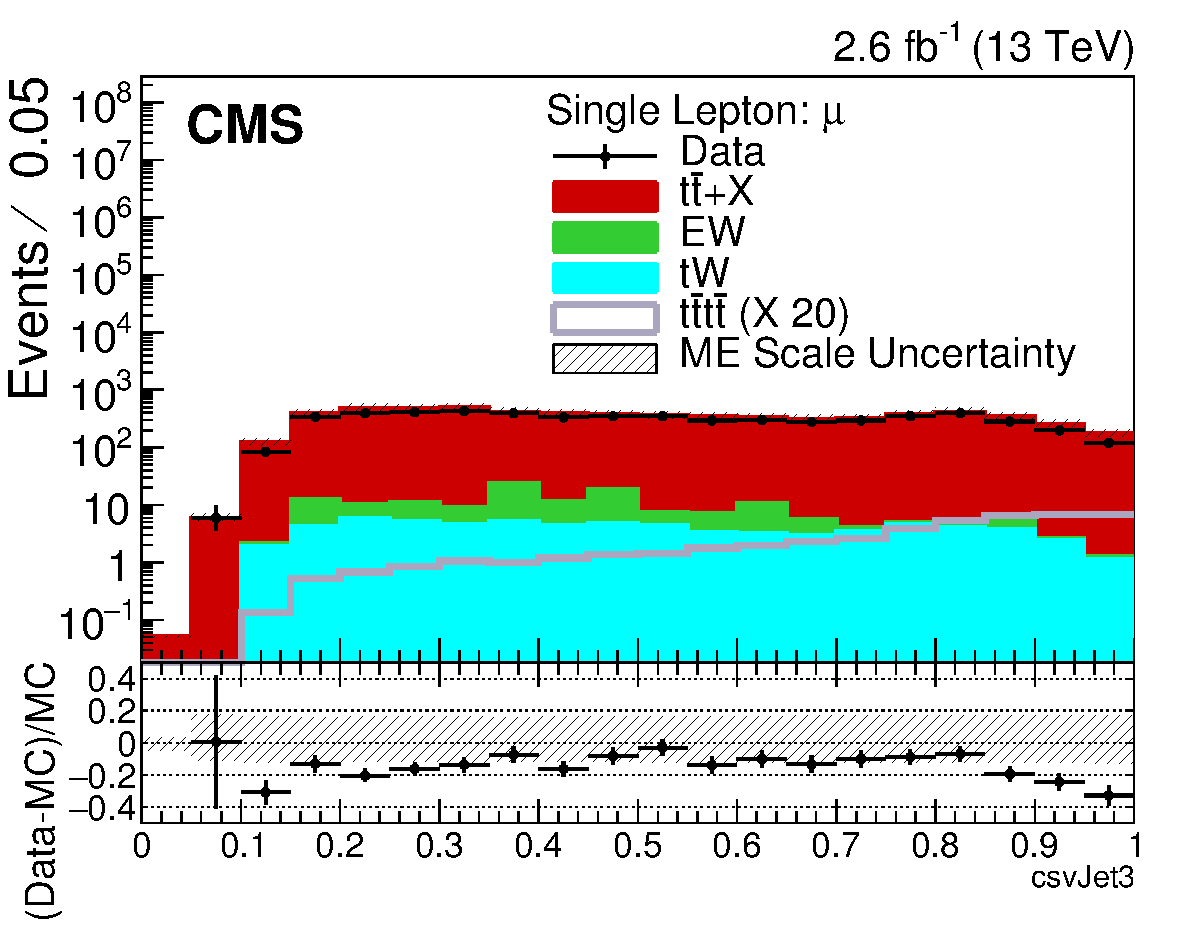
\includegraphics[width=0.44\textwidth]{images/Run2/csvJet3_StackLogY_noSF.pdf}
    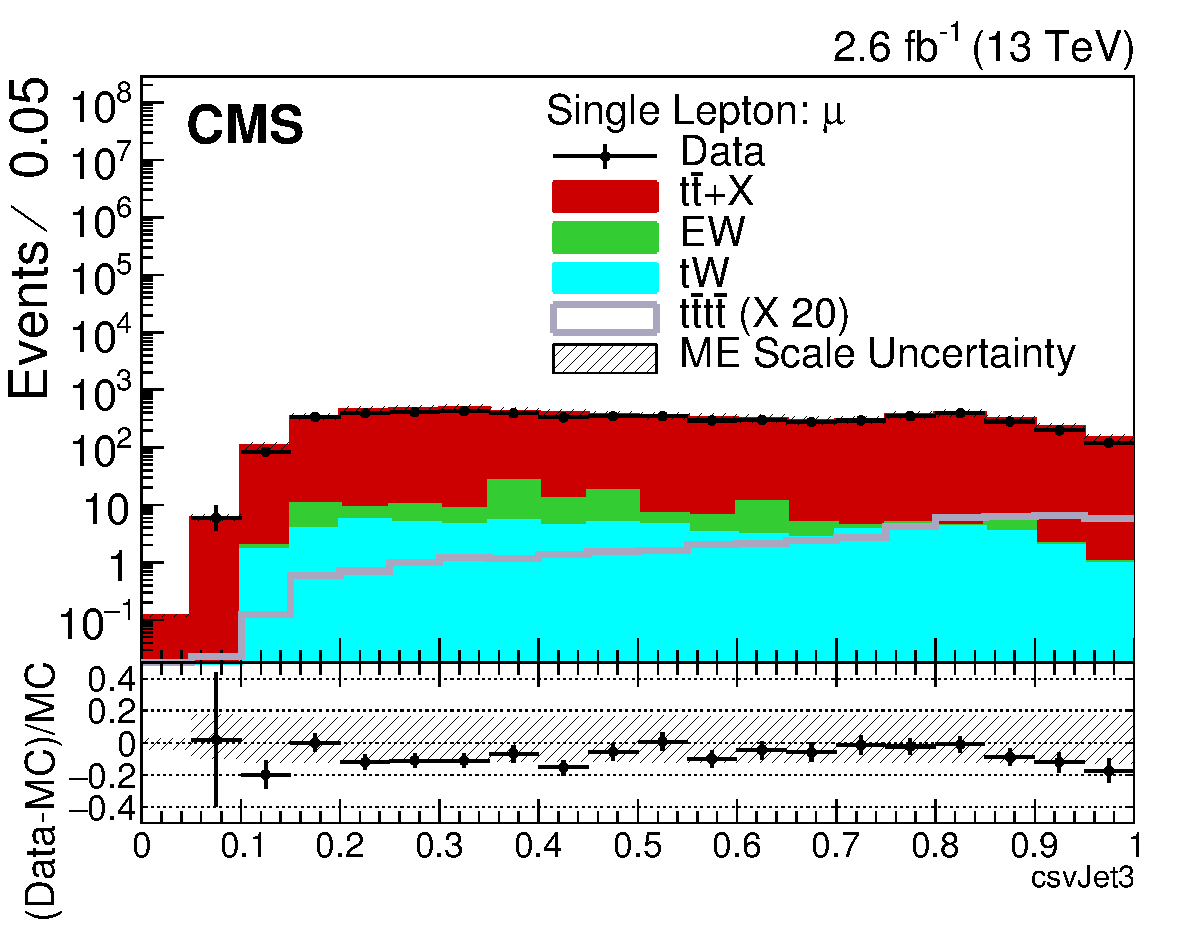
\includegraphics[width=0.44\textwidth]{images/Run2/csvJet3_StackLogY.pdf}
    \caption{ The third-highest ranked CSV jet distributions for data and simulation event in the $\mu$ + jets channel (left) and $e$ + jets channel (right) are plotted.}
    \label{fig:csvJet3SF}
\end{figure}
\begin{figure}[ht!]
    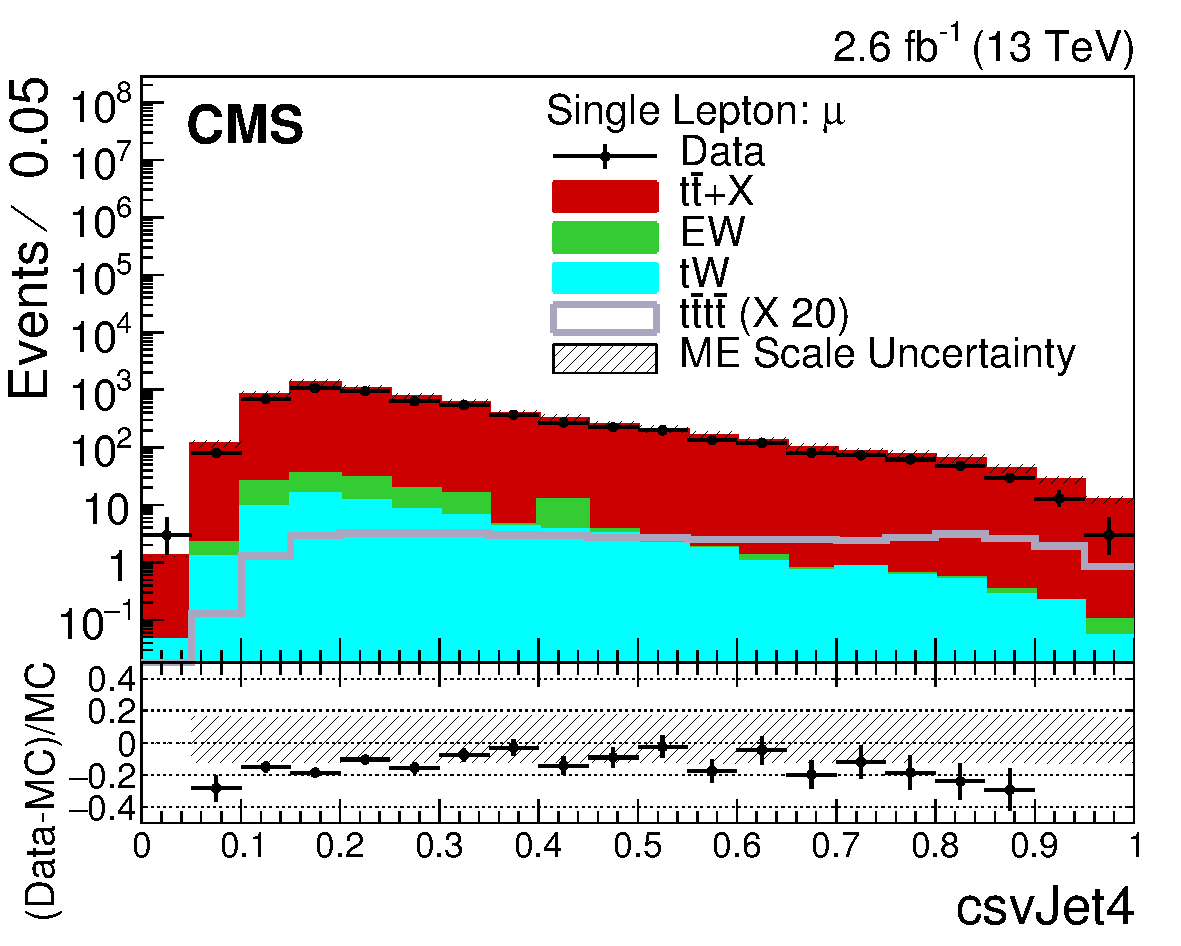
\includegraphics[width=0.44\textwidth]{images/Run2/csvJet4_StackLogY_noSF.pdf}
    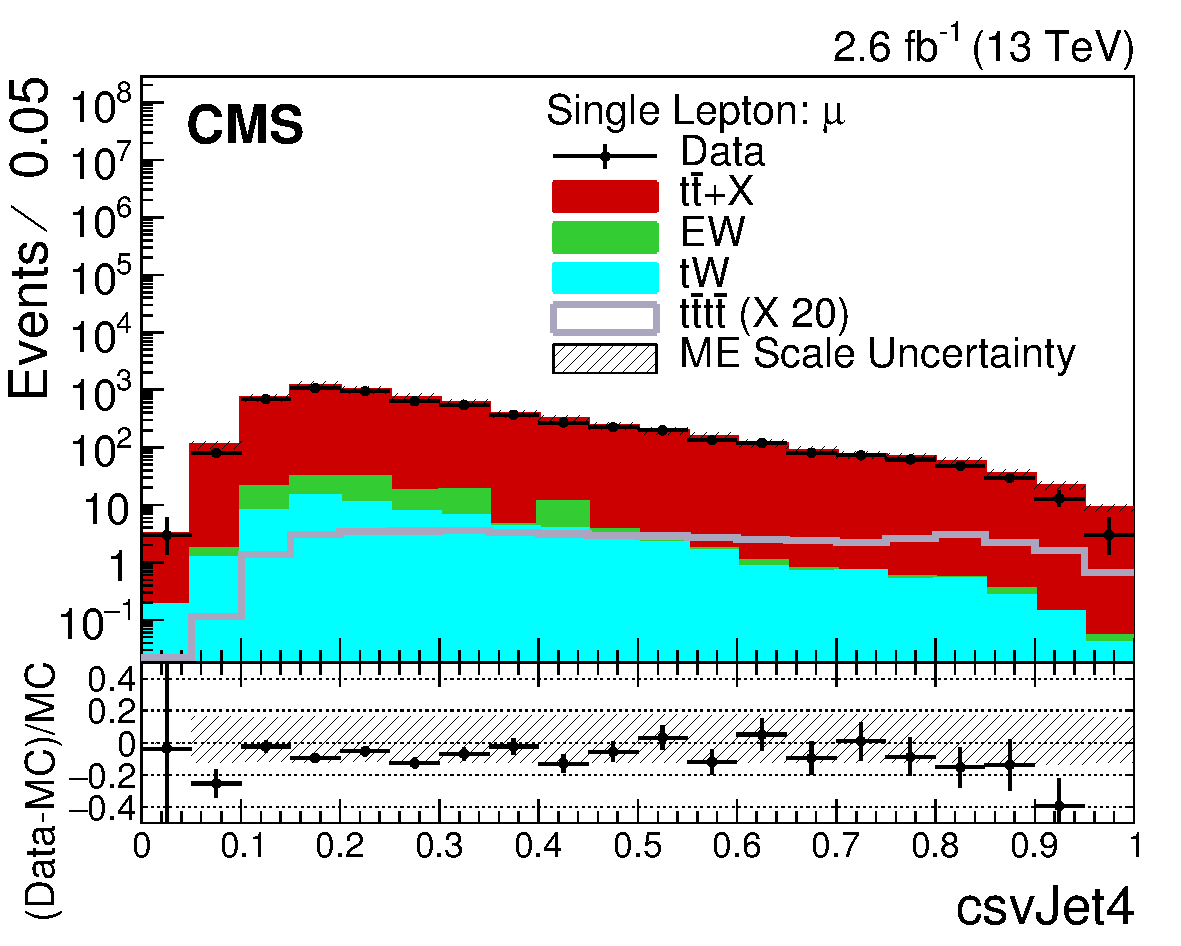
\includegraphics[width=0.44\textwidth]{images/Run2/csvJet4_StackLogY.pdf}
    \caption{ The fourth-highest ranked CSV jet distributions for data and simulation event in the $\mu$ + jets channel (left) and $e$ + jets channel (right) are plotted.}
    \label{fig:csvJet4SF}
\end{figure}

\begin{figure}[h!]
\begin{center}
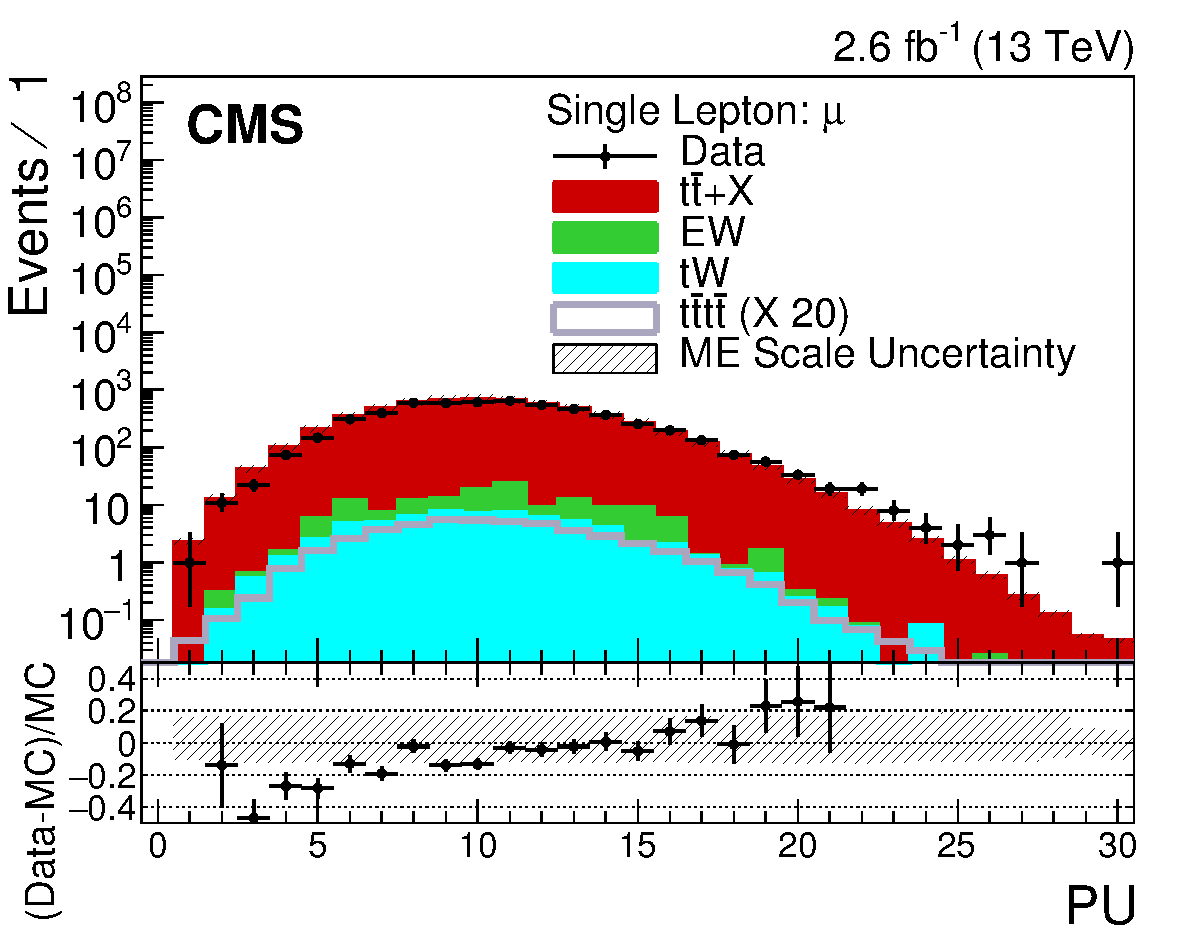
\includegraphics[width=0.67\textwidth]{images/Run2/PU_StackLogY.pdf}
\end{center}
\caption{The number of primary vertices for data and simulation after re-weighting for mu + jets.}
\label{fig:PUReWeight13}
\end{figure} 

The jet multiplicity modelling from section~\ref{subsec:alphaS} was applied. It can be seen from Figs.~\ref{fig:withAlpha} and~\ref{fig:withoutAlpha} that the jet multiplicity modelling is greatly improved by applying this correction.

\begin{figure}[ht!]
    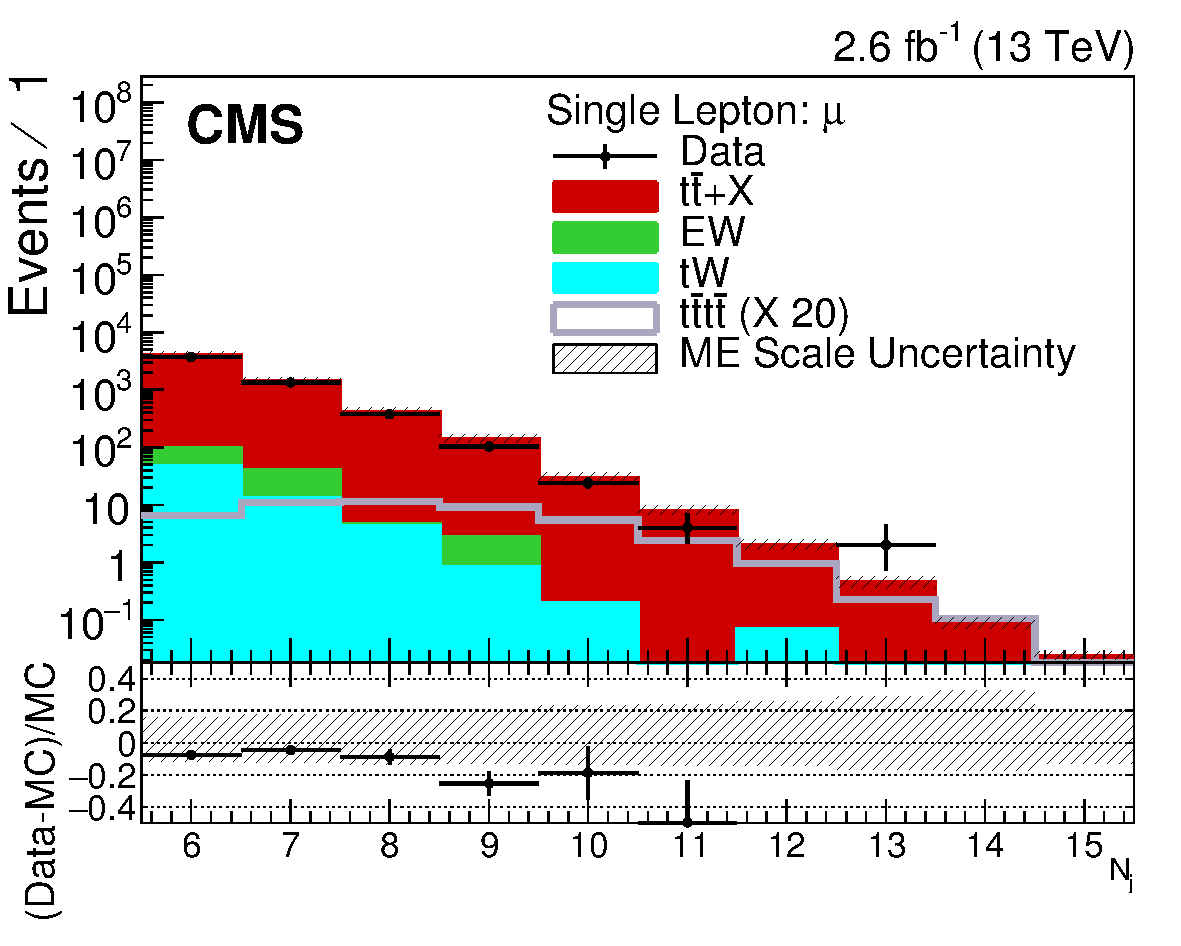
\includegraphics[width=0.48\textwidth]{images/Run2/nJets_StackLogY.pdf}
    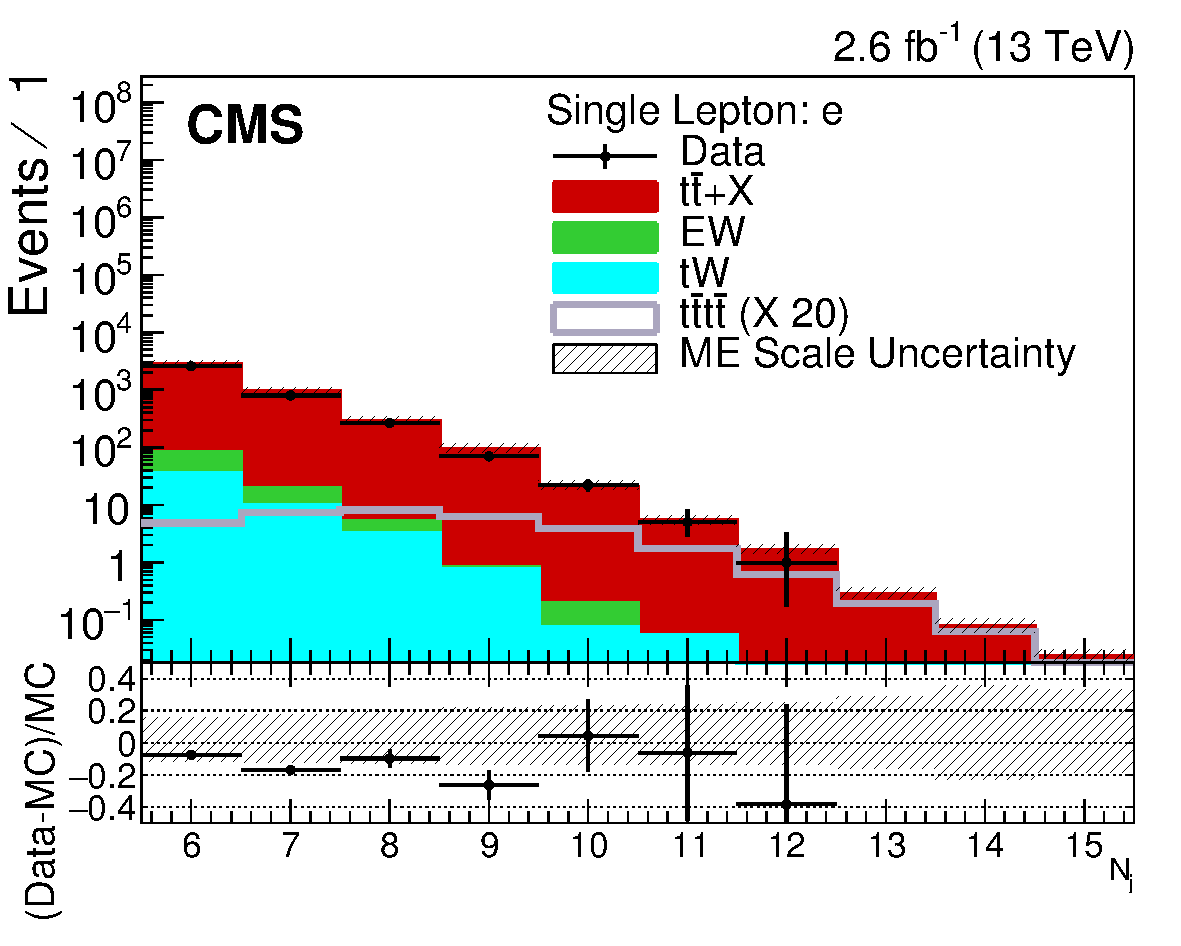
\includegraphics[width=0.48\textwidth]{images/Run2/nJets_StackLogY_e.pdf}
    \caption{The \njets distributions for data and simulation in the $\mu$ + jets channel (left) and $e$ + jets channel (left) with jet multiplicity modelling scale factors applied.}
    \label{fig:withAlpha}
\end{figure}

\begin{figure}[ht!]
    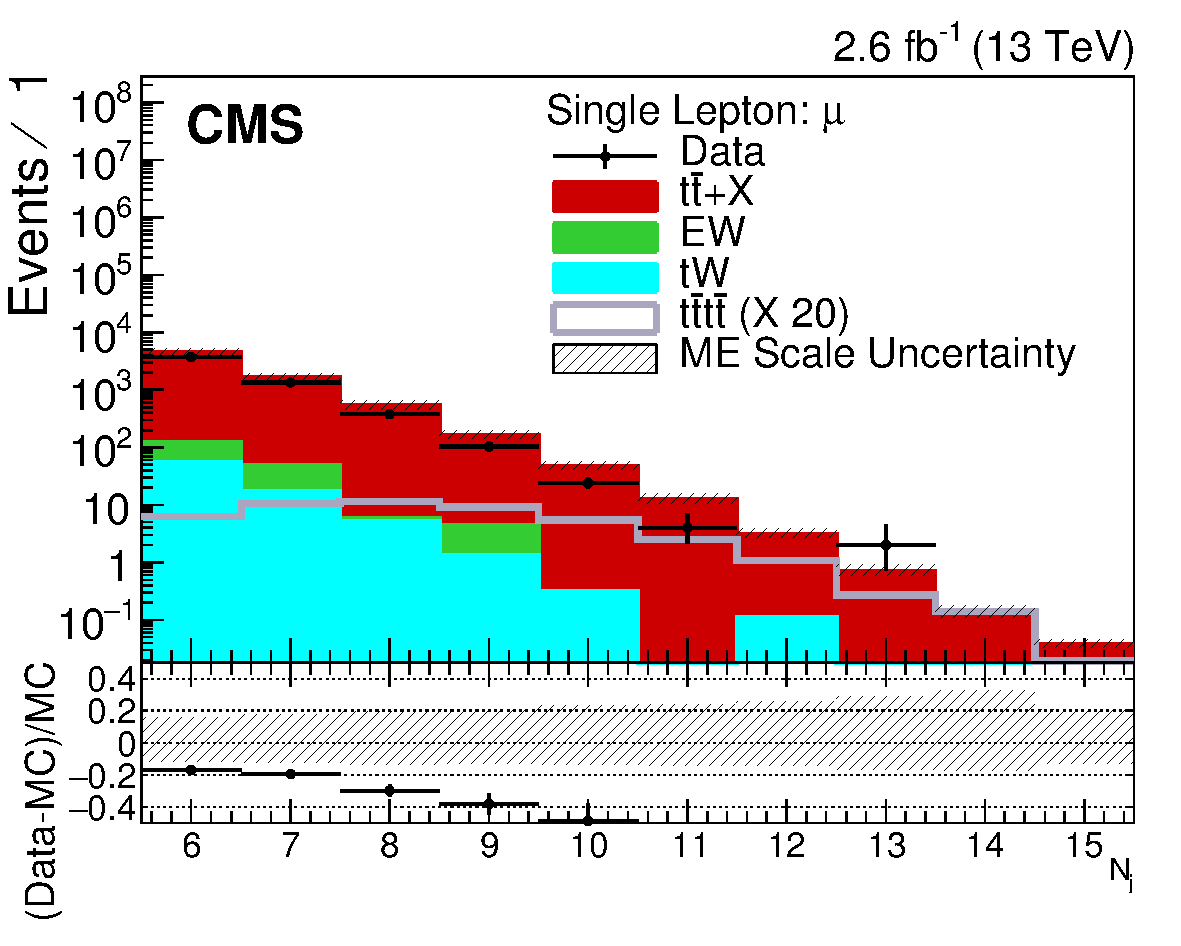
\includegraphics[width=0.48\textwidth]{images/Run2/nJets_StackLogY_woAlphaS.pdf}
    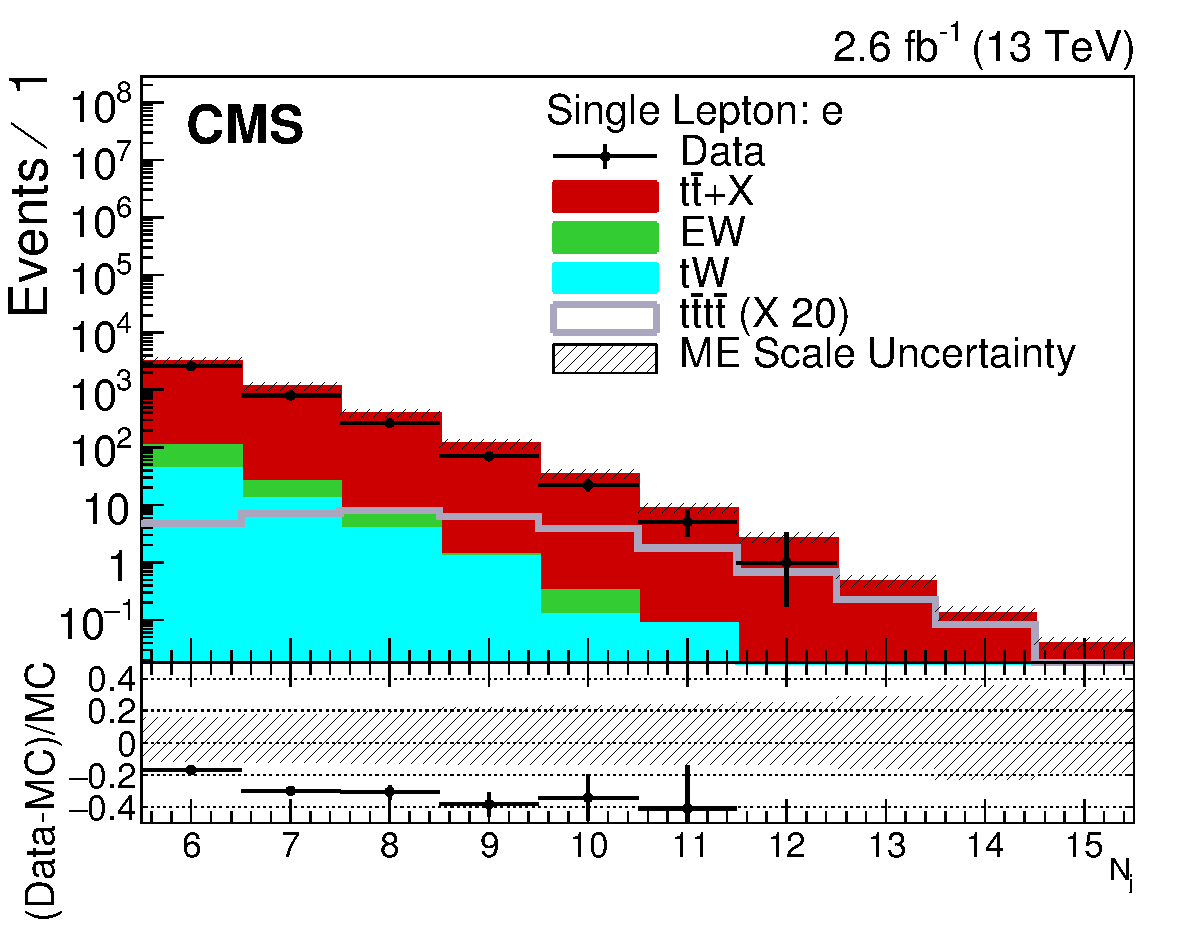
\includegraphics[width=0.48\textwidth]{images/Run2/nJets_StackLogY_e_woAlphaS.pdf}
    \caption{The \njets distributions for data and simulation in the $\mu$ + jets channel (left) and $e$ + jets channel (left) without jet multiplicity modelling scale factors applied.}
    \label{fig:withoutAlpha}
\end{figure}

The scale factors applied for the heavy flavour modelling are described in Section~\ref{ttbbmod}. The distributions for the \nMtags are shown with and without the heavy flavour modelling scale factors applied. It is not obvious that there is a significant improvement in the \nMtags after the scale factors have been applied but the heavy flavour fraction is allowed to float as a shape nuisance parameter in the template fit.

\begin{figure}[ht!]
    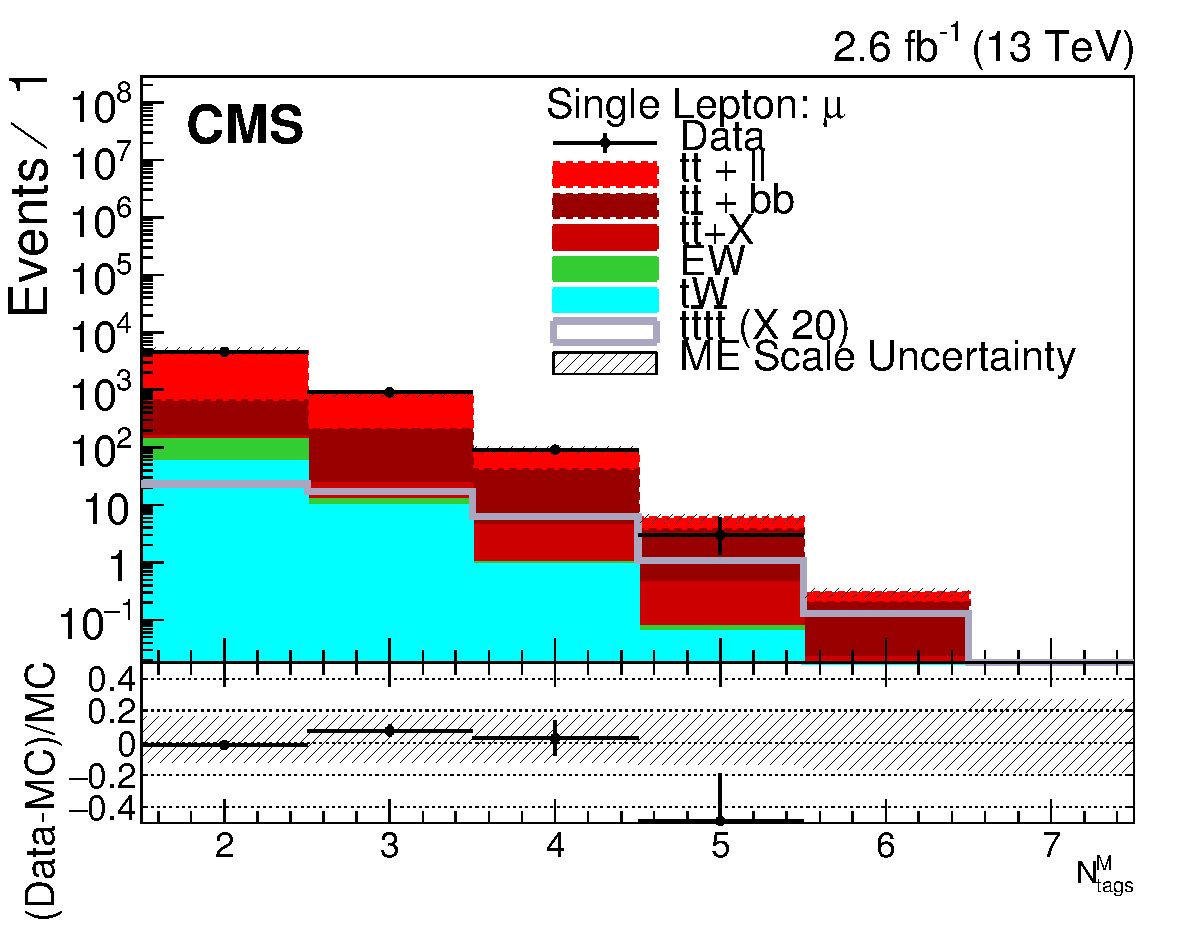
\includegraphics[width=0.47\textwidth]{images/Run2/nMtags_StackLogY_HF_wo_reweight.pdf} 
    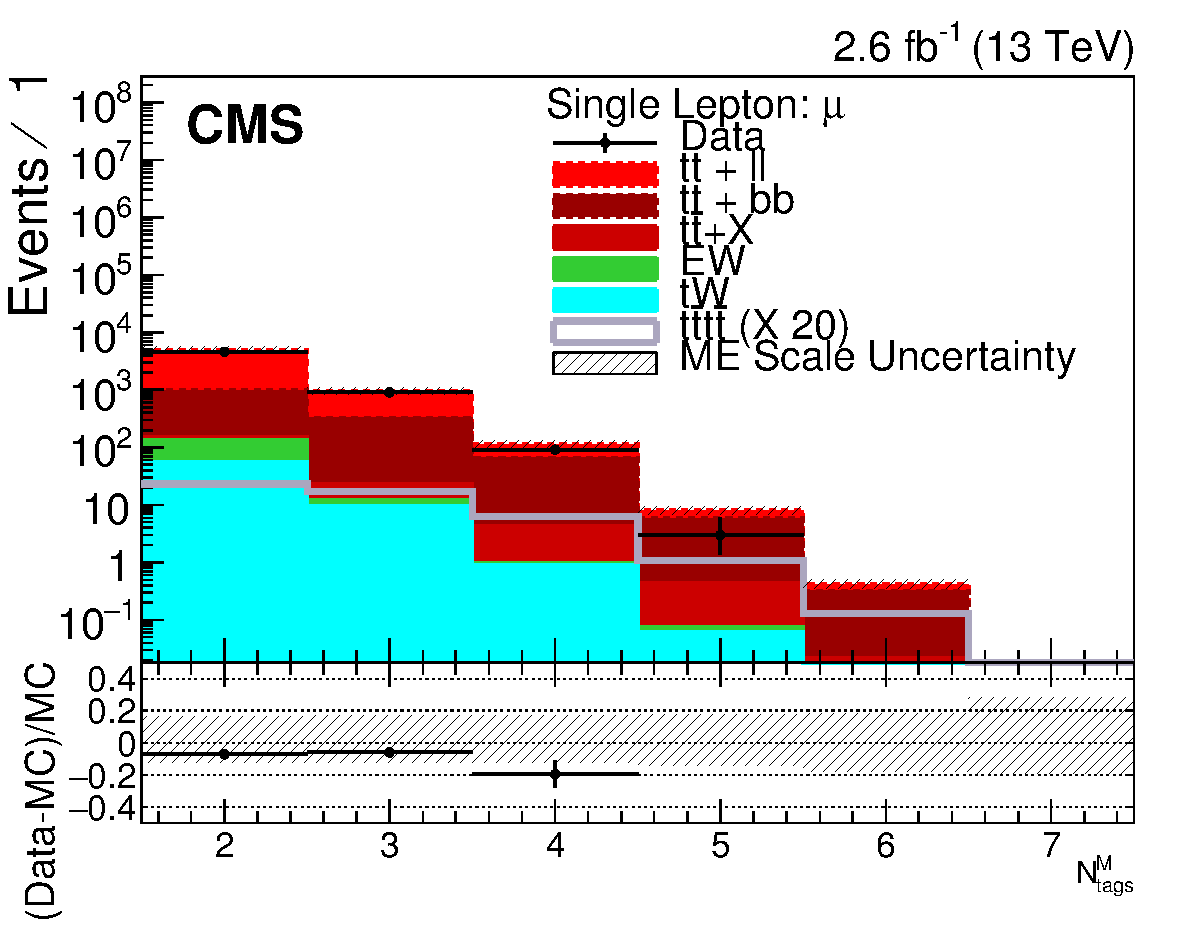
\includegraphics[width=0.47\textwidth]{images/Run2/nMtags_StackLogY_HF_w_reweight.pdf} 
    \caption{\nMtags are shown for the muon channel with heavy flavour reweighting (right) and without(left).}
    \label{fig:HF_reweight}
\end{figure}

\section{Weighted event counts at each baseline event selection requirement \label{cutflow13}}

\section{Data-simulation agreement}

\section{Discriminating between signal and background}
\label{sec:discriminating13}

It can be seen in Section~\ref{cutflow13} that the \ttbar background is three orders of magnitude larger in the signal region. The variables used to discriminate between \ttbar and \tttt are described below.
% There are three main features which can be used to discriminate; the number of top quarks which can be reconstructed in the event, the number of b-jets found in each event, and event activity such as \HT.

\subsection{Hadronic top quark content}
\label{sec:topContent13}

As the \antikt algorithm cannot resolve jets which have $\Delta R = \sqrt{  \theta^{2} + \phi^{2} } < 0.4$, a hadronically decaying top quark can only be deemed \emph{reconstructible} if the minimal $\Delta R$ between all three jets is $> 0.4$ which happens $> 98\%$ of the time in \ttbar and \tttt simulation when studying the decay products of leptons and partons, and pairs of partons.\\
The BDT training was performed on 273~K \ttbar events. The input variables to the hadronic top quark reconstruction BDT are shown in Fig.~\ref{fig:TrijetBDTInputFeatures13}. The separation power for each of these variables and for the output BDT discriminator distribution in Fig.~\ref{fig:TrijetBDTOutput13} is evident as in the \runone chapter. 

\begin{figure}[ht!]
\centering
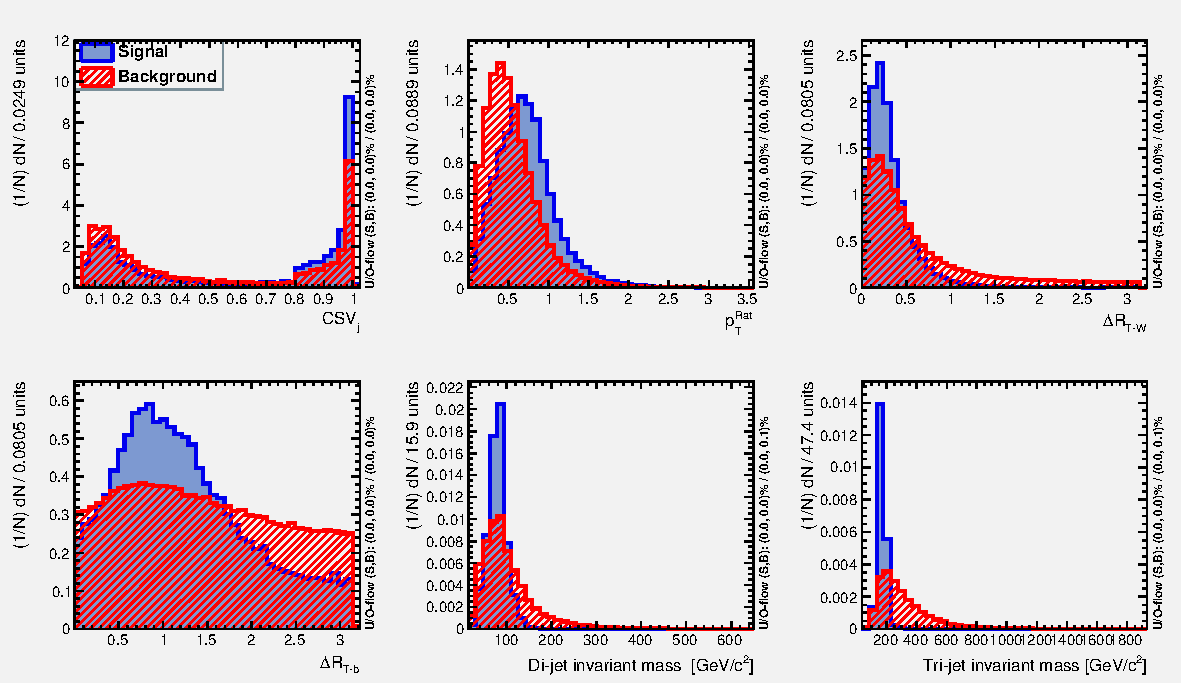
\includegraphics[width=\linewidth]{images/Run2/variables_id_c1.pdf}
\caption{Normalised distributions of the six variables used the MVA hadronic Top kinematic reconstruction are shown for good (red histograms) and bad (blue histograms) trijets.}
\label{fig:TrijetBDTInputFeatures13}
\end{figure}

\begin{figure}[ht!]
\begin{center}
    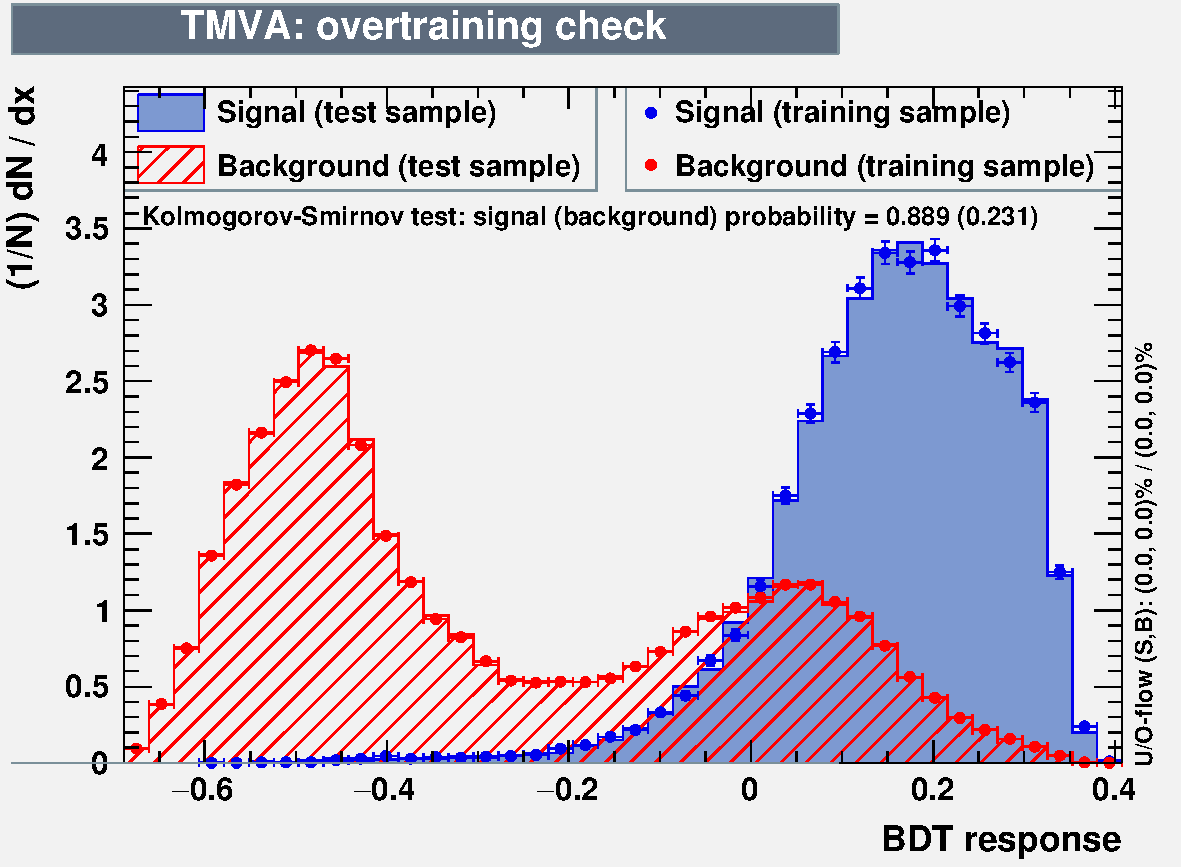
\includegraphics[width=0.55\textwidth]{images/Run2/overtrain_BDT.pdf}
    \caption{The discriminator distributions for the BDT classifier for good and bad trijets in training and validation samples.}
    \label{fig:TrijetBDTOutput13}
\end{center}
\end{figure}

The affect of the tri-jet invariant mass variable in the BDT is shown in Fig.~\ref{fig:multimode13} where it can be clearly seen that this variable contributes to the strong splitting of the BDT output distribution at a value of $\approx-0.2$.

\begin{figure}[ht!]
\begin{center}
    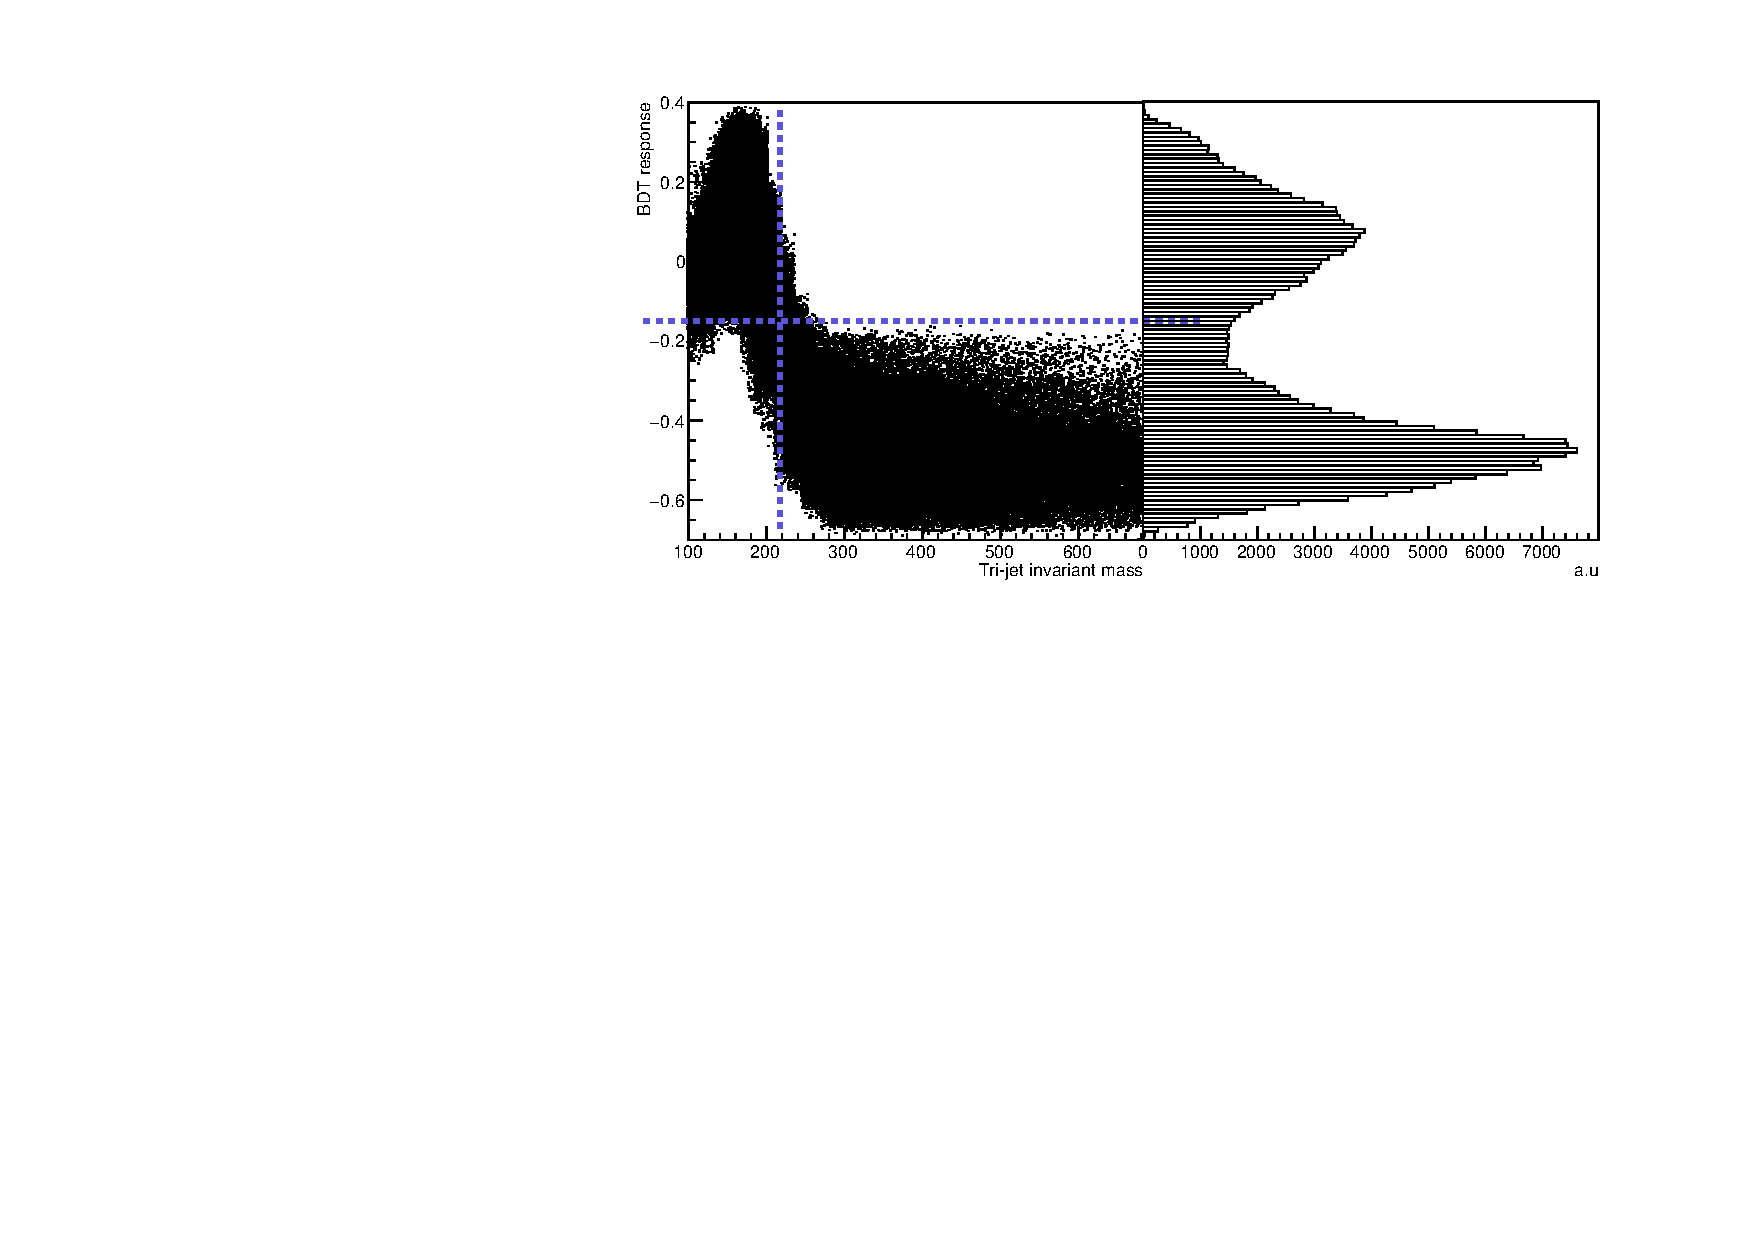
\includegraphics[width=0.85\textwidth]{images/Run2/multimode.pdf}
    \caption{The discriminator distributions for the BDT classifier versus trijet invariant mass and the projection on the vertical axis. Dashed lines indicate the cut value on trijet invariant mass at the BDT root node.}
    \label{fig:multimode13}
\end{center}
\end{figure}

In Fig.~\ref{fig:ContoursTopMassHadrWmass13}, the left-hand plot shows the distribution of good and bad tri-jet combinations in the phase space of tri-jet and di-jet invariant mass. It can be seen from the right-hand plot in Fig.~\ref{fig:ContoursTopMassHadrWmass13} that high BDT discriminator values are found in the region where the good tri-jet combinations are clustered.
\begin{figure}[ht!]
\begin{center}
    \includegraphics[width=\textwidth]{images/Run2/ContoursHadrWmassTopMass.pdf}
    \caption{(Left)  Di-jet versus trijet invariant mass distribution for good (blue) and bad (red) trijet combinations. (Right) The average BDT response as a function of Di-jet versus trijet invariant mass input variables.}
    \label{fig:ContoursTopMassHadrWmass13}
\end{center}
\end{figure}

\subsubsection*{BDT$_{tri-jet2}$}

The distribution for BDT$_{tri-jet2}$ is shown in Fig.~\ref{fig:bdtTrijet213}. There is good agreement between the data and simulation and sufficient discrimination power to be used in the event-level BDT.

\begin{figure}[ht!]
    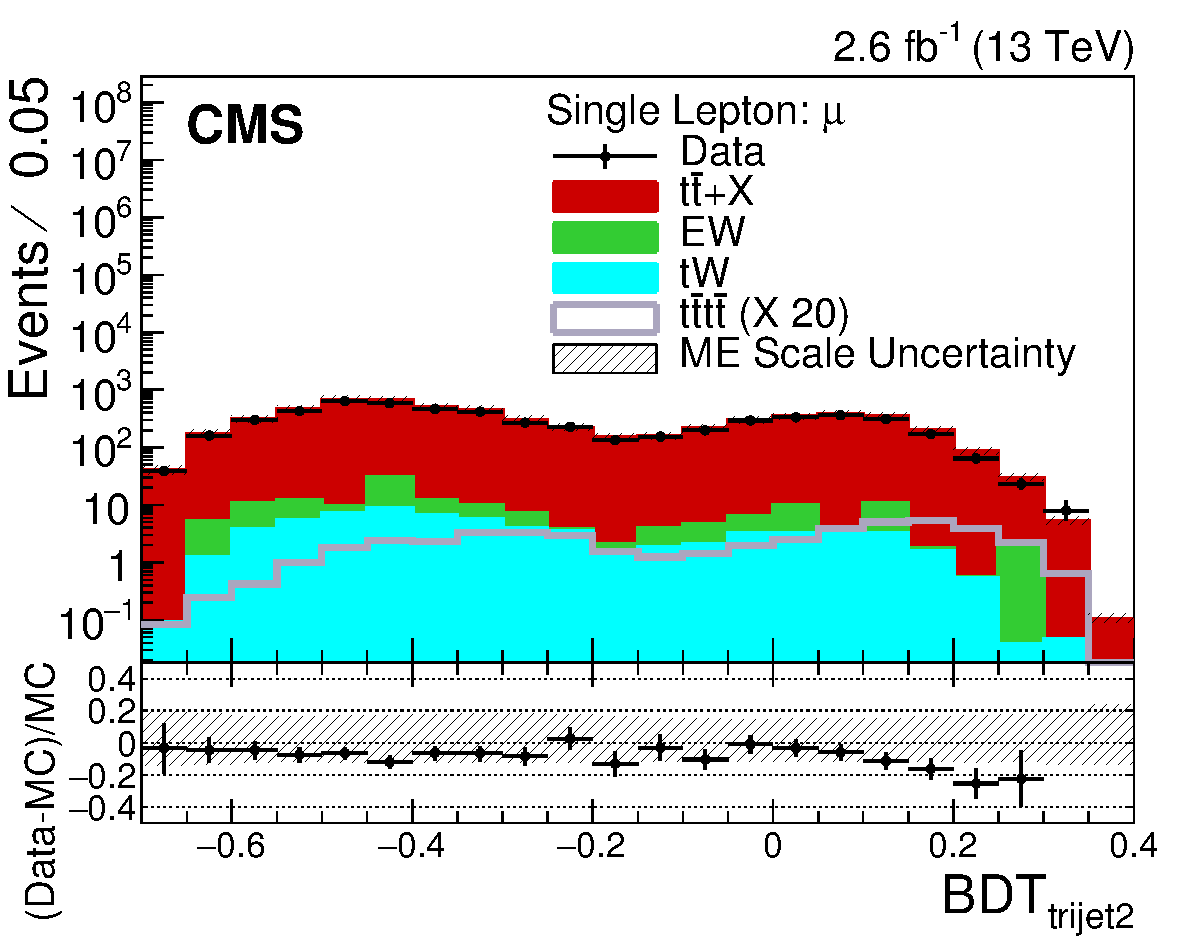
\includegraphics[width=0.44\textwidth]{images/Run2/BDT_trijet2_StackLogY.pdf}
    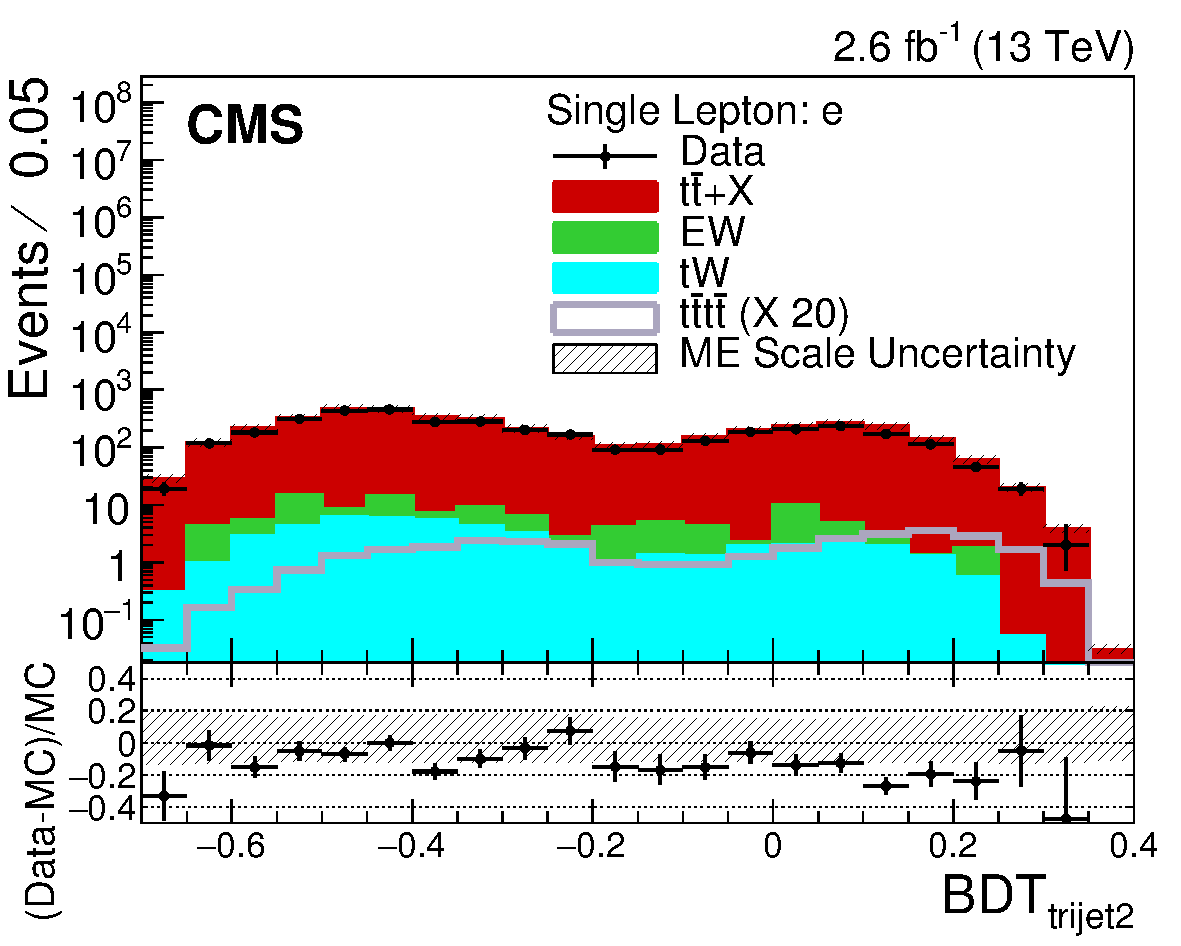
\includegraphics[width=0.44\textwidth]{images/Run2/BDT_trijet2_StackLogY_e.pdf}
    \caption{ The BDT$_{trijet2}$ distributions for data and simulation event in the $\mu$ + jets channel (left) and $e$ + jets channel (right) are plotted.}
    \label{fig:bdtTrijet213}
\end{figure}

\subsubsection*{Reduced Event Variables}
The reduced variables formed from the reduced event, where the jets from the highest-ranked hadronic top quark have been removed from the collection of jets, are shown in Figs.~\ref{fig:htx13} and~\ref{fig:sumjetmassx13}. Again, good agreement is observed between the data and simulation and both variables were found to have good discrimination power in the event-level BDT.

\begin{figure}[ht!]
    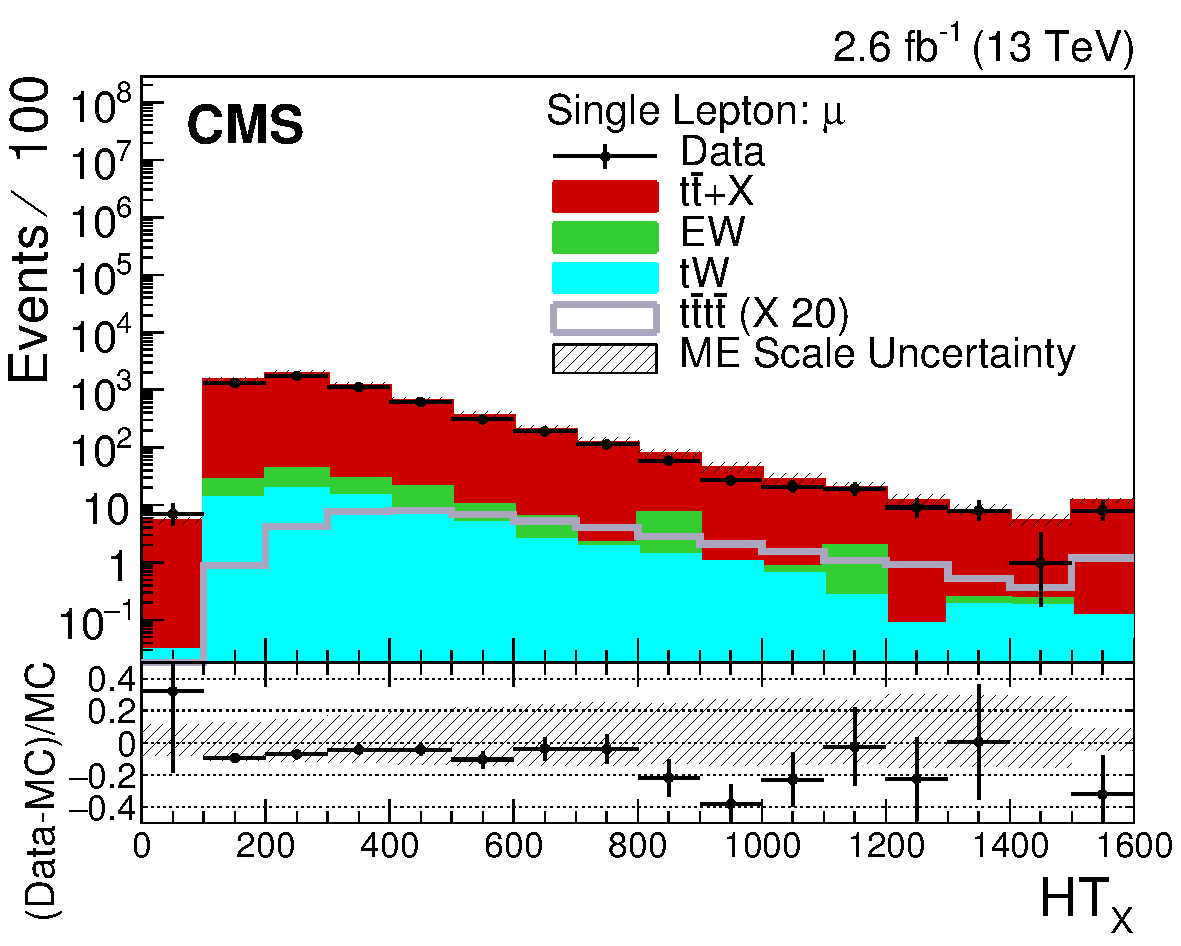
\includegraphics[width=0.44\textwidth]{images/Run2/HTX_StackLogY.pdf}
    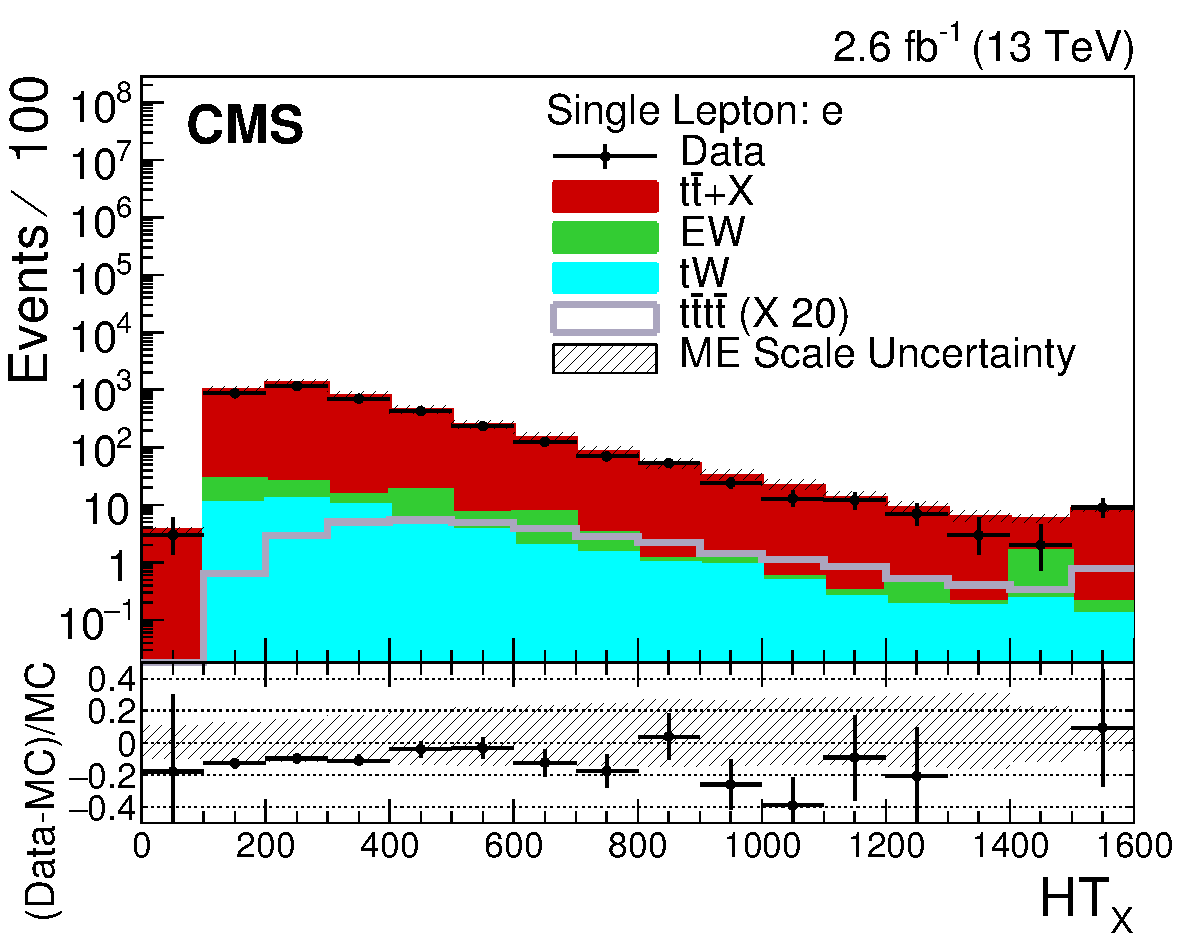
\includegraphics[width=0.44\textwidth]{images/Run2/HTX_StackLogY_e.pdf}
    \caption{ The \HTX distributions for data and simulation event in the $\mu$ + jets channel (left) and $e$ + jets channel (right) are plotted.}
    \label{fig:htx13}
\end{figure}

\begin{figure}[ht!]
    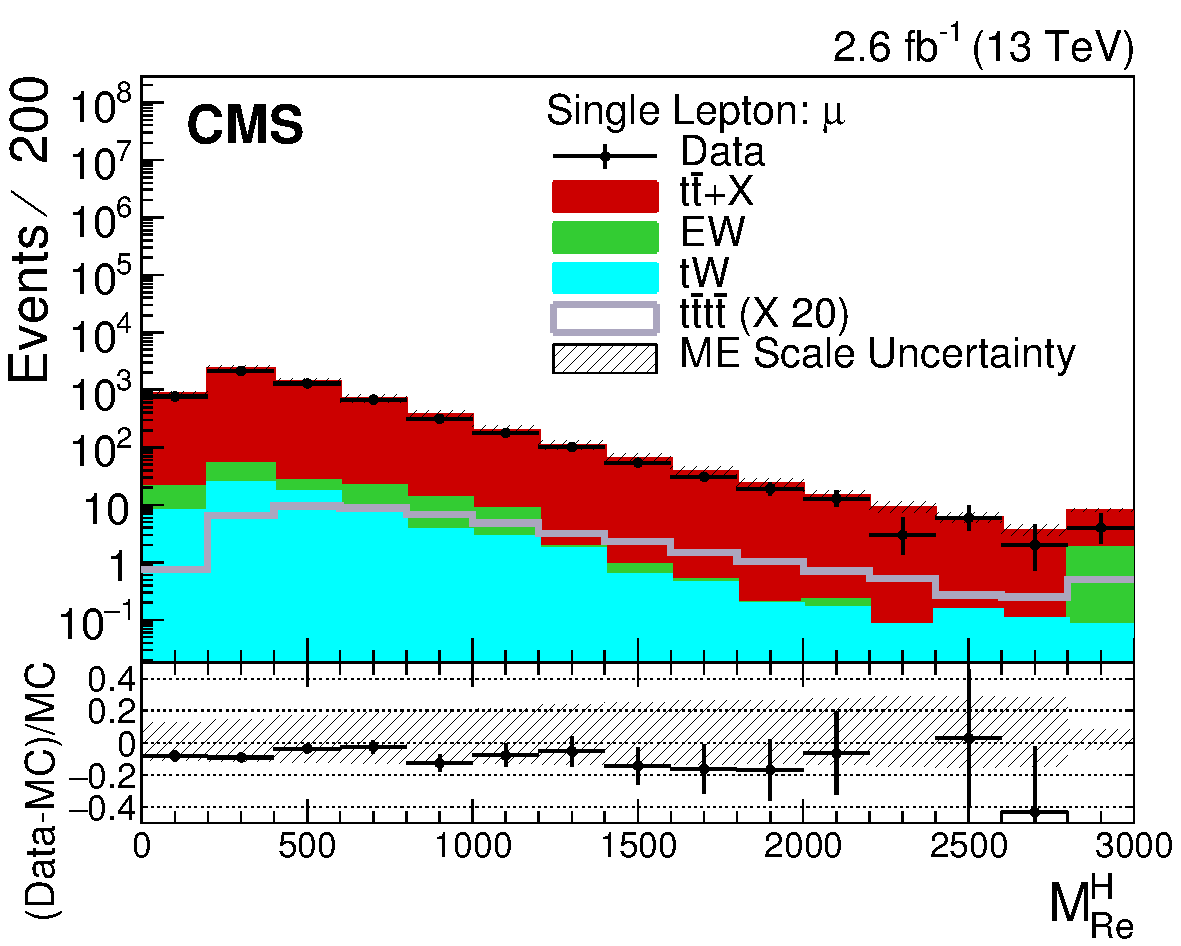
\includegraphics[width=0.44\textwidth]{images/Run2/SumJetMassX_StackLogY.pdf}
    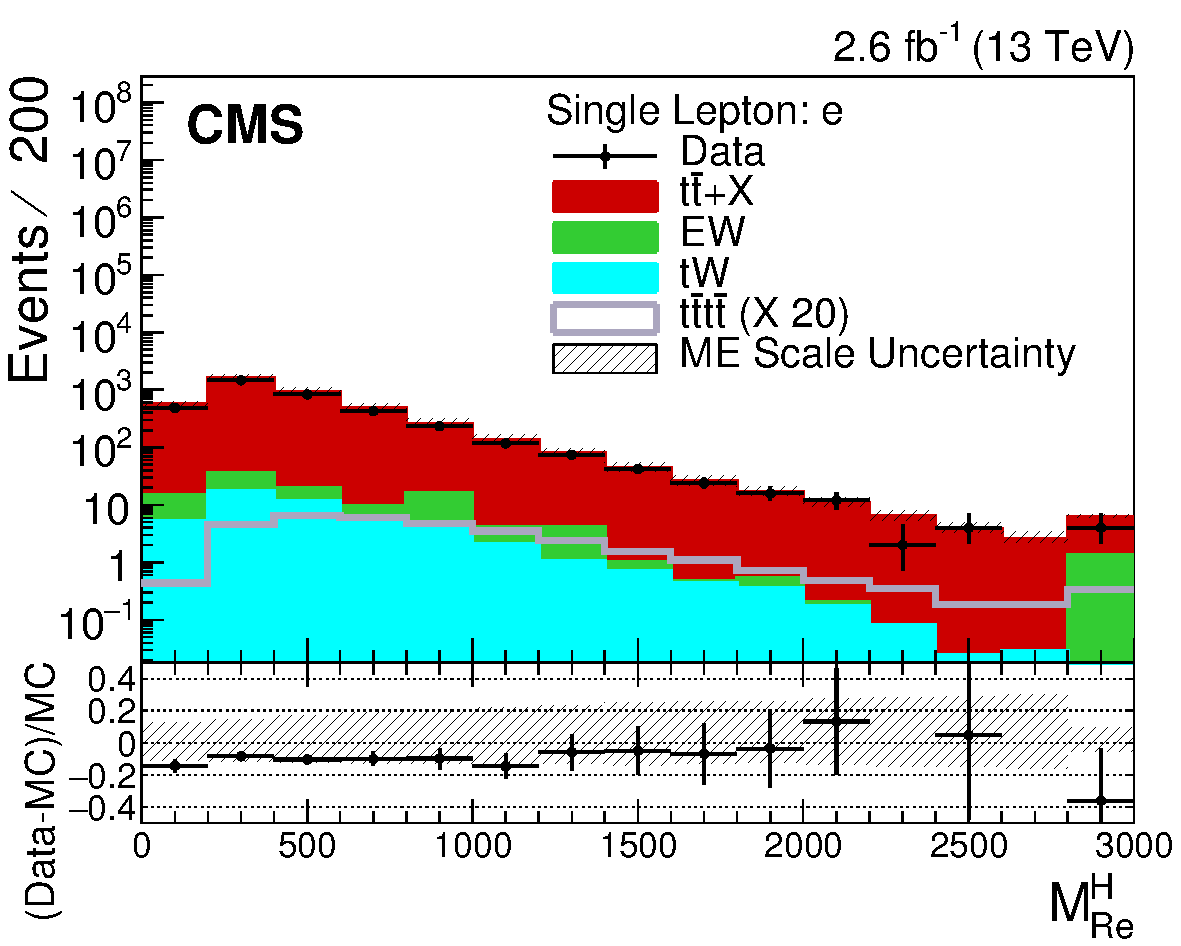
\includegraphics[width=0.44\textwidth]{images/Run2/SumJetMassX_StackLogY_e.pdf}
    \caption{ The \redhadmass distributions for data and simulation event in the $\mu$ + jets channel (left) and $e$ + jets channel (right) are plotted.}
    \label{fig:sumjetmassx13}
\end{figure}


\subsection{Event activity and b-jet content variables chosen for the event-level BDT}
The following variables were chosen for their discrimination power within the event-level BDT and are previously described in section~\ref{sec:Strategy}. It should be noted that the third-highest CSV and fourth-highest CSV values can be used in the $\sqrt{s} = 13$~TeV analysis as the CSV distributions have been corrected by the modelling in section~\ref{subsec:method2btag}.


\begin{multicols}{2}
\setlength{\columnseprule}{0pt} 

\begin{itemize}
\item \htb
\item \htrat
\item \njets
\item lepton \pt, \leadleppt
\item \njetsw
\item third-highest CSV
\item fourth-highest CSV
\end{itemize}

\end{multicols}

\subsection{Event-level BDT}
A \ttbar sample and a \tttt sample is provided to the TMVA package to train and test the performance of the event-level BDT using the AdaBoost boosting algorithm~\cite{FREUND1997119} was used. The \MADGRAPH\aMCATNLO \tttt sample was used with all \fxnote{are neg weights described anywhere}{negative weights} set to one in the training. The gradient boosting algorithm~\cite{mason1999boosting} can be used with negative weights hence it was used to verify that the inclusion of negative weights (or not) had negligible impact on the final limit. Ultimately the AdaBoost algorithm produced a stronger limit on the \tttt cross section than the gradient boosting algorithm with the negative weights set to one. The jet modelling scale factor weight from Section~\ref{subsec:alphaS} is supplied to the BDT as it is important to correct the mismodelling of the most powerful variable input into the BDT.\\
The separation of the input variables, before any boost weights are applied, is shown in Fig.~\ref{fig:BDTInputVars} and the ranking of the variables in terms of variable importance are shown for the muon channel in table~\ref{tab:BDTrankings}. The variables \njets, third-highest CSV and \htrat are the highest ranked variables and their discriminating power is evident in their initial separation power. The lowest ranked variable is \leadleppt, which is also seen in Fig.~\ref{fig:BDTInputVars} to have poor separation power initially. However it still enhances the discrimination power of the BDT to include the \leadleppt variable and it is preferable to have at least one leptonic variable in the list of input variables rather than all hadronic variables.


\fixme{gradboost studies}
\fixme{training studies..separate jet cats, tree numbers, min node size}
\fixme{jets+tags categories studies}


\begin{figure}[h!]
    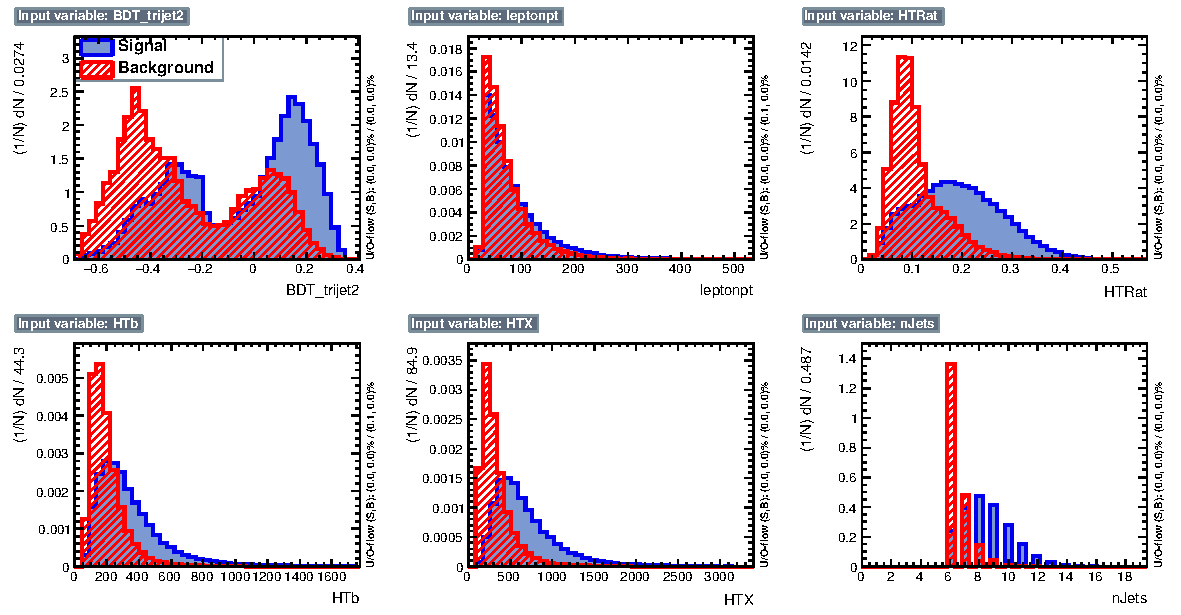
\includegraphics[width=\textwidth]{images/Run2/variables_id_c1_ELBDT13.pdf}\\
    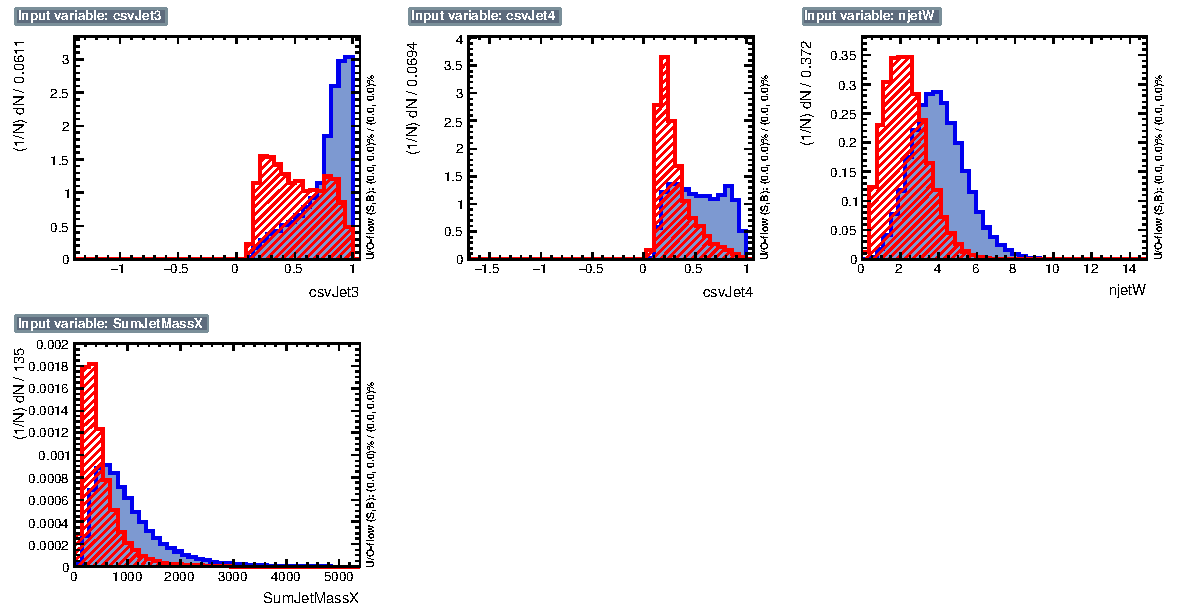
\includegraphics[width=\textwidth]{images/Run2/variables_id_c2_ELBDT13.pdf}
    \caption{Normalised distributions of the input variables in the muon channel taken from TMVA}
    \label{fig:BDTInputVars}
\end{figure}

\begin{table}[ht!]
\centering
\begin{tabular}{| l | l | l | p{5cm} |}
  \hline
Rank & Variable & Importance \\
 \hline
1 & \njets & 1.340e-01\\
2 & third-highest CSV &1.180e-01\\
3 & \htrat & 1.133e-01\\
4 & BDT$_{trijet2}$ & 1.091e-01 \\
5 & \njetsw &1.082e-01\\
6 & \redhadmass& 1.026e-01\\
7 & \HTX & 9.867e-02\\
8 & \htb & 8.650e-02 \\
9 & fourth-highest CSV & 7.630e-02\\
10 & \leadleppt & 5.334e-02  \\
\hline
\end{tabular}
 \caption{Ranking of variables in order of discrimination power within the BDT.}
  \label{tab:BDTrankings}
  \end{table}

The output discriminator value for the event level BDT is split into \njets categories of 6, 7, 8 and $\geq$9 jets and further to the \runone analysis in Chapter~\ref{c:Run1}, the distributions are also split into \nMtags categories of 2, 3 and $\geq$4 b-tags which further splits the distributions into regions which are more sensitive to the signal and regions which are better for constraining the background.
The output pre-fit BDT plots are shown in \njets and \nMtags categories in Figs.~\ref{fig:BDT_Mu29Aug400trees_5MinNodeSize_20nCuts_3MaxDepth_5adaboostbeta_adaBoost_alphaSTune_noMinEvents62}~-~\ref{fig:BDT_Mu29Aug400trees_5MinNodeSize_20nCuts_3MaxDepth_5adaboostbeta_adaBoost_alphaSTune_noMinEvents94}. It can be seen that the signal becomes more separated from the background in the higher \njets and \nMtags categories as it move towards higher BDT discriminator values. The lower \njets and \nMtags categories can help to constrain the \ttbar background. These categories act like control region due to the very large background to signal ratio.

\begin{figure}[ht!]
    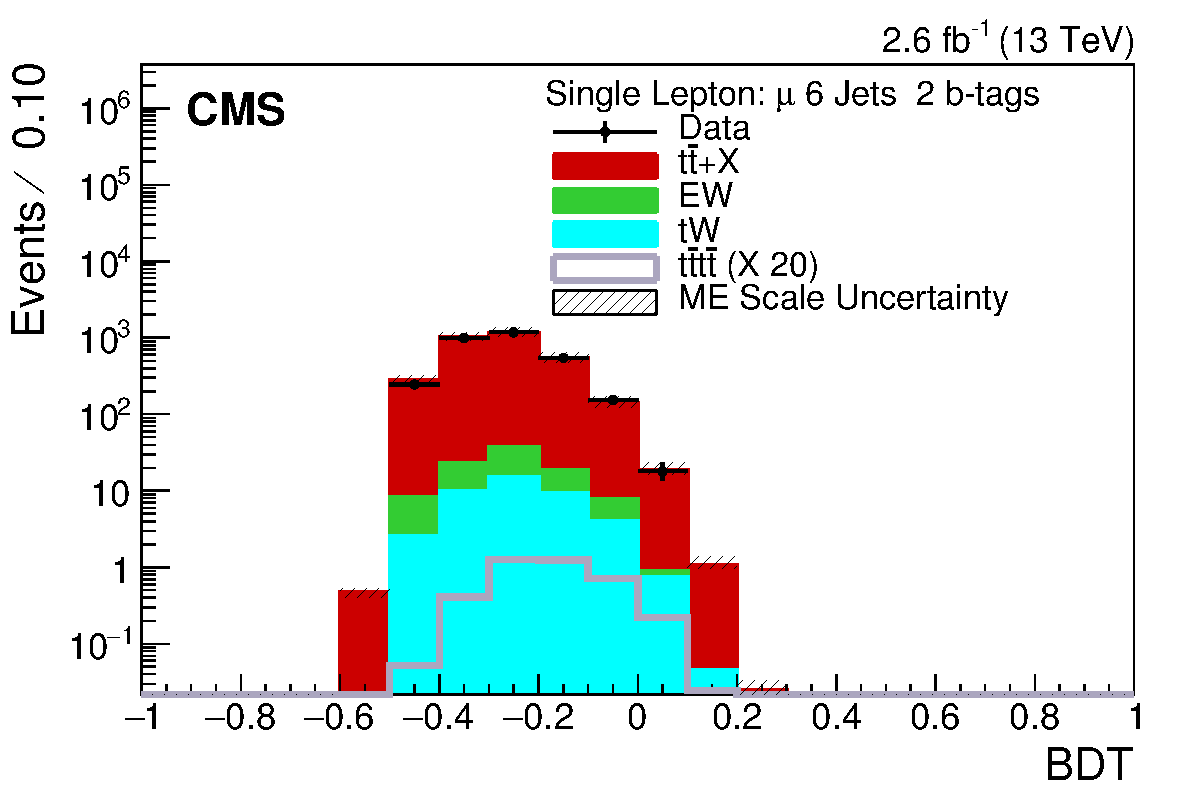
\includegraphics[width=0.48\textwidth]{images/Run2/BDT_Mu29Aug400trees_5MinNodeSize_20nCuts_3MaxDepth_5adaboostbeta_adaBoost_alphaSTune_noMinEvents6nJets2nMtags_StackLogY.pdf}
    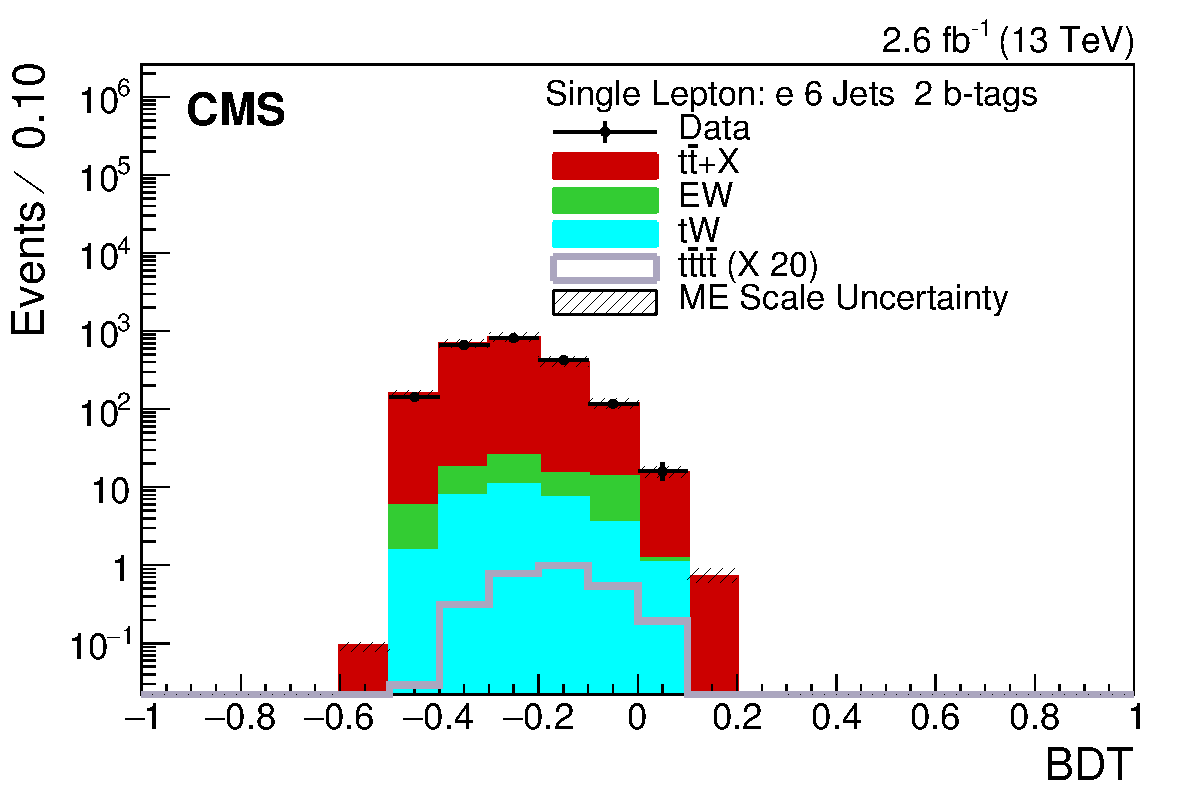
\includegraphics[width=0.48\textwidth]{images/Run2/BDT_El29Aug400trees_5MinNodeSize_20nCuts_3MaxDepth_5adaboostbeta_adaBoost_alphaSTune_noMinEvents6nJets2nMtags_StackLogY.pdf} 
    \caption{The BDT output distributions for AdaBoost for data and simulation in the $\mu$ + jets channel (left) and e + jets channel (left) are shown for the 6 \njets and 2\nMtags category.}
    \label{fig:BDT_Mu29Aug400trees_5MinNodeSize_20nCuts_3MaxDepth_5adaboostbeta_adaBoost_alphaSTune_noMinEvents62}
\end{figure}

\begin{figure}[ht!]
    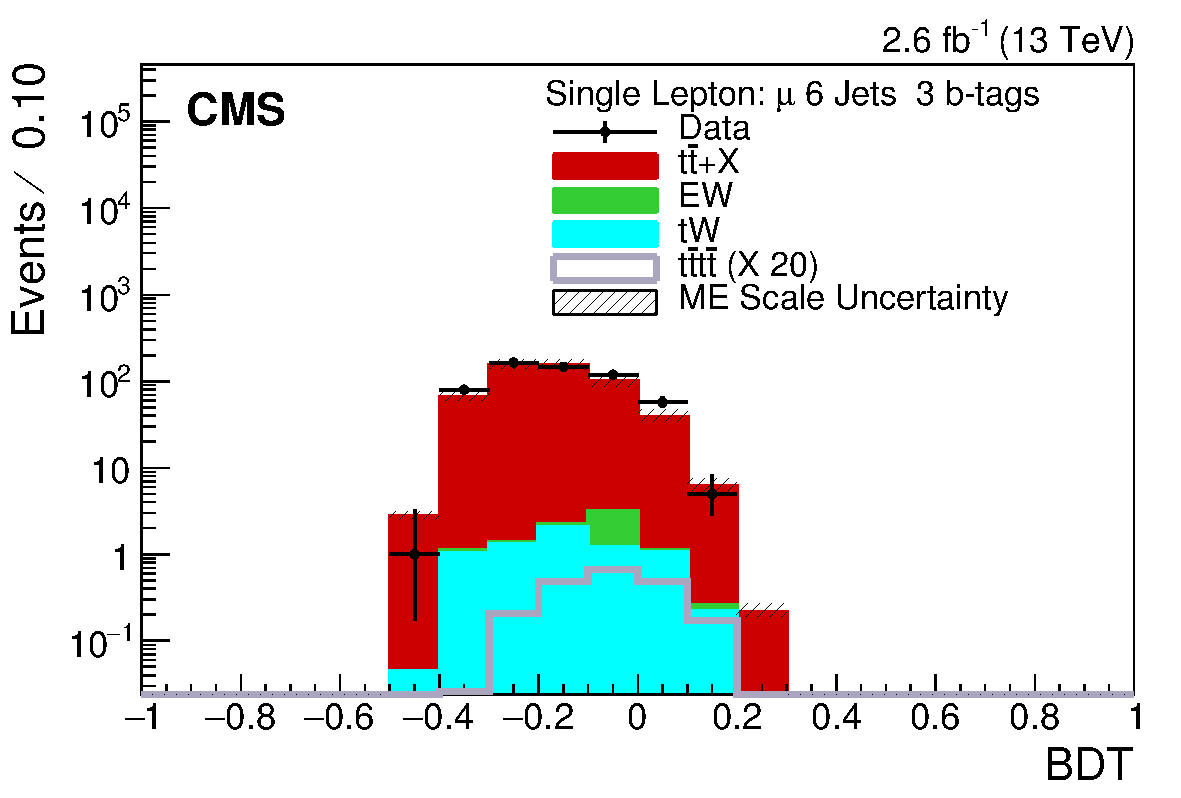
\includegraphics[width=0.48\textwidth]{images/Run2/BDT_Mu29Aug400trees_5MinNodeSize_20nCuts_3MaxDepth_5adaboostbeta_adaBoost_alphaSTune_noMinEvents6nJets3nMtags_StackLogY.pdf}
    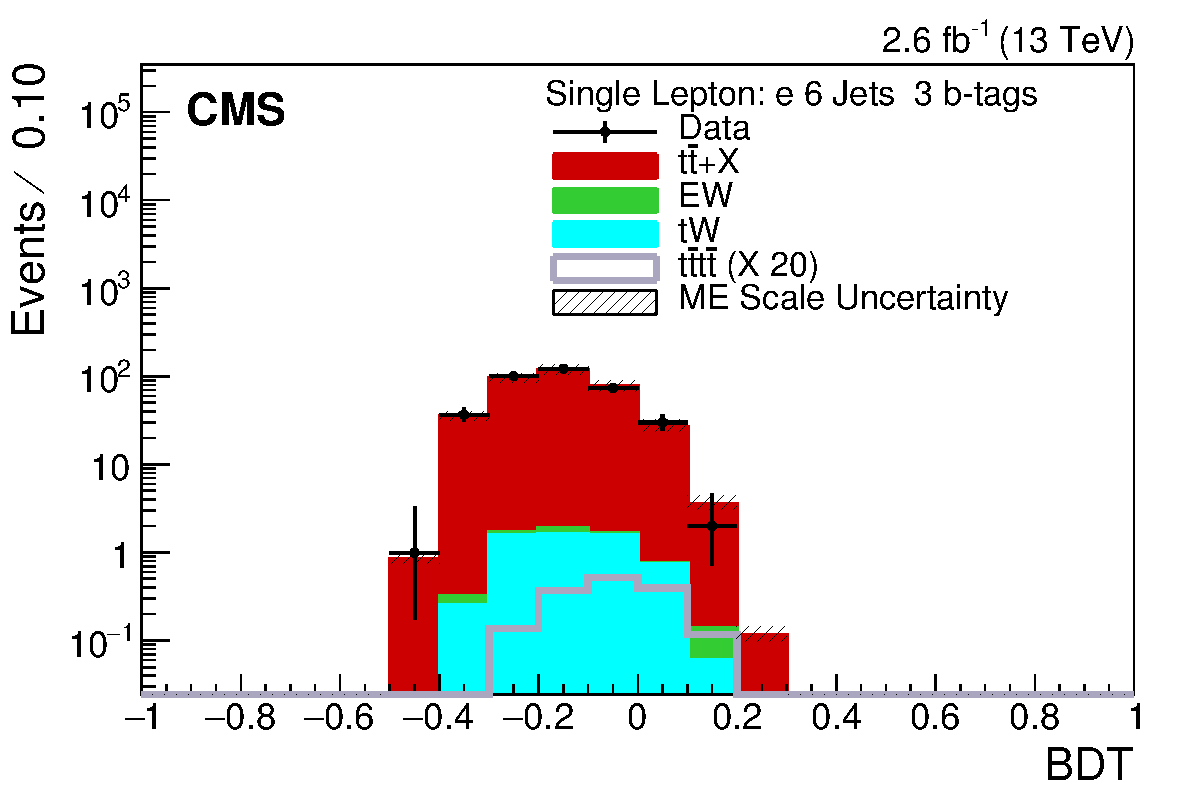
\includegraphics[width=0.48\textwidth]{images/Run2/BDT_El29Aug400trees_5MinNodeSize_20nCuts_3MaxDepth_5adaboostbeta_adaBoost_alphaSTune_noMinEvents6nJets3nMtags_StackLogY.pdf} 
    \caption{The BDT output distributions for AdaBoost for data and simulation in the $\mu$ + jets channel (left) and e + jets channel (left) are shown for the 6 \njets and 3\nMtags category.}
    \label{fig:BDT_Mu29Aug400trees_5MinNodeSize_20nCuts_3MaxDepth_5adaboostbeta_adaBoost_alphaSTune_noMinEvents63}
\end{figure}

\begin{figure}[ht!]
    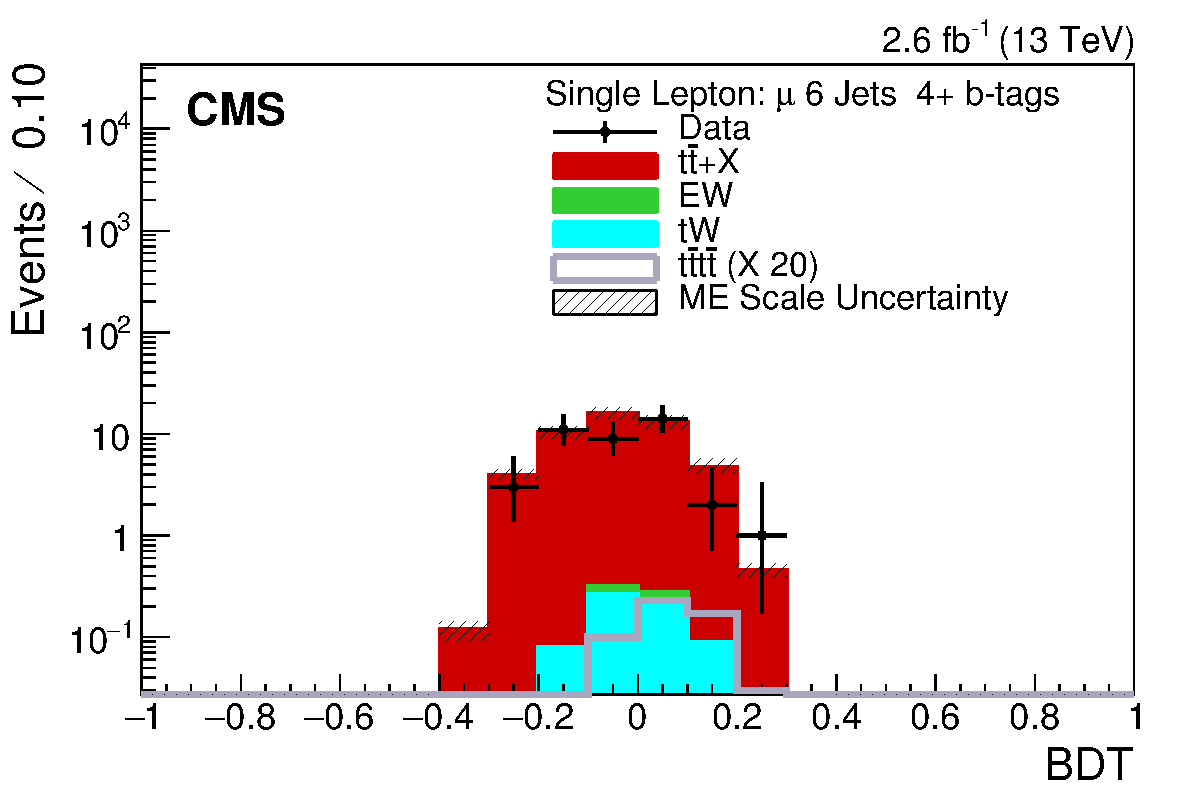
\includegraphics[width=0.48\textwidth]{images/Run2/BDT_Mu29Aug400trees_5MinNodeSize_20nCuts_3MaxDepth_5adaboostbeta_adaBoost_alphaSTune_noMinEvents6nJets4nMtags_StackLogY.pdf}
    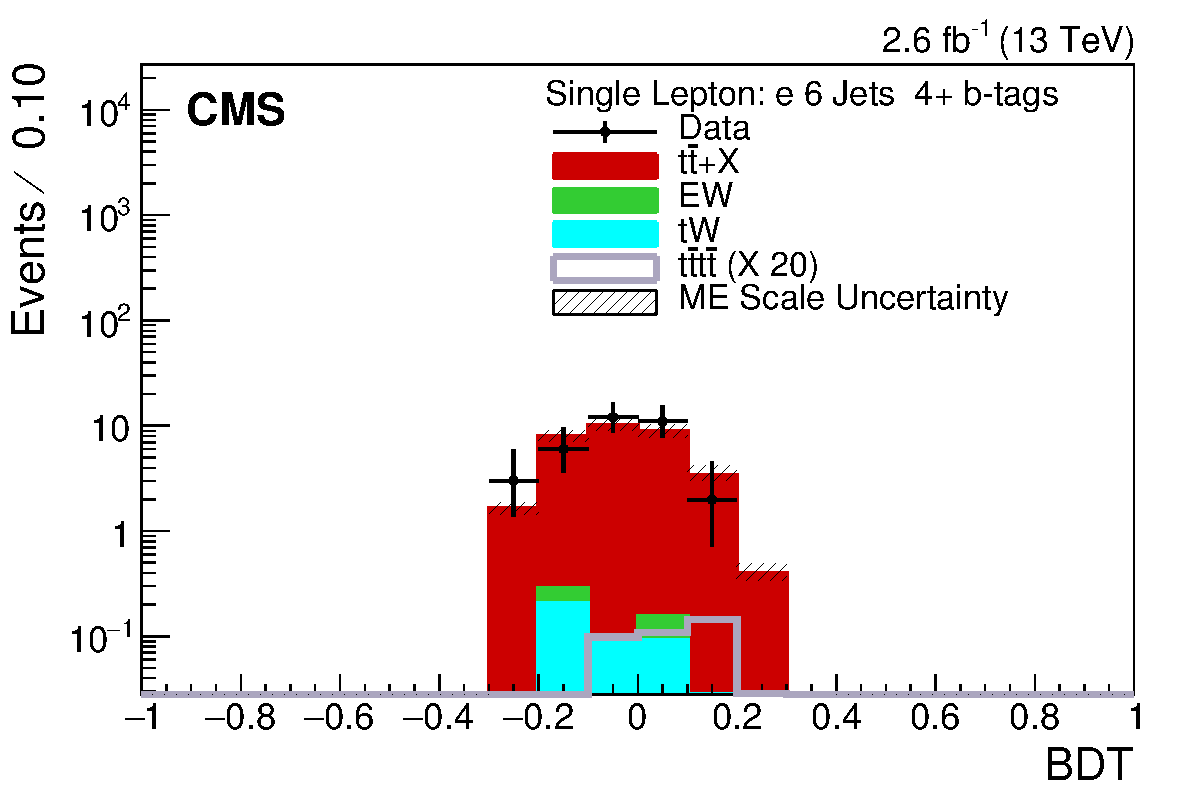
\includegraphics[width=0.48\textwidth]{images/Run2/BDT_El29Aug400trees_5MinNodeSize_20nCuts_3MaxDepth_5adaboostbeta_adaBoost_alphaSTune_noMinEvents6nJets4nMtags_StackLogY.pdf}
    \caption{The BDT output distributions for AdaBoost for data and simulation in the $\mu$ + jets channel (left) and e + jets channel (right) are shown for the 6 \njets and $\geq4$ \nMtags category.}
    \label{fig:BDT_Mu29Aug400trees_5MinNodeSize_20nCuts_3MaxDepth_5adaboostbeta_adaBoost_alphaSTune_noMinEvents64}
\end{figure}

\begin{figure}[ht!]
    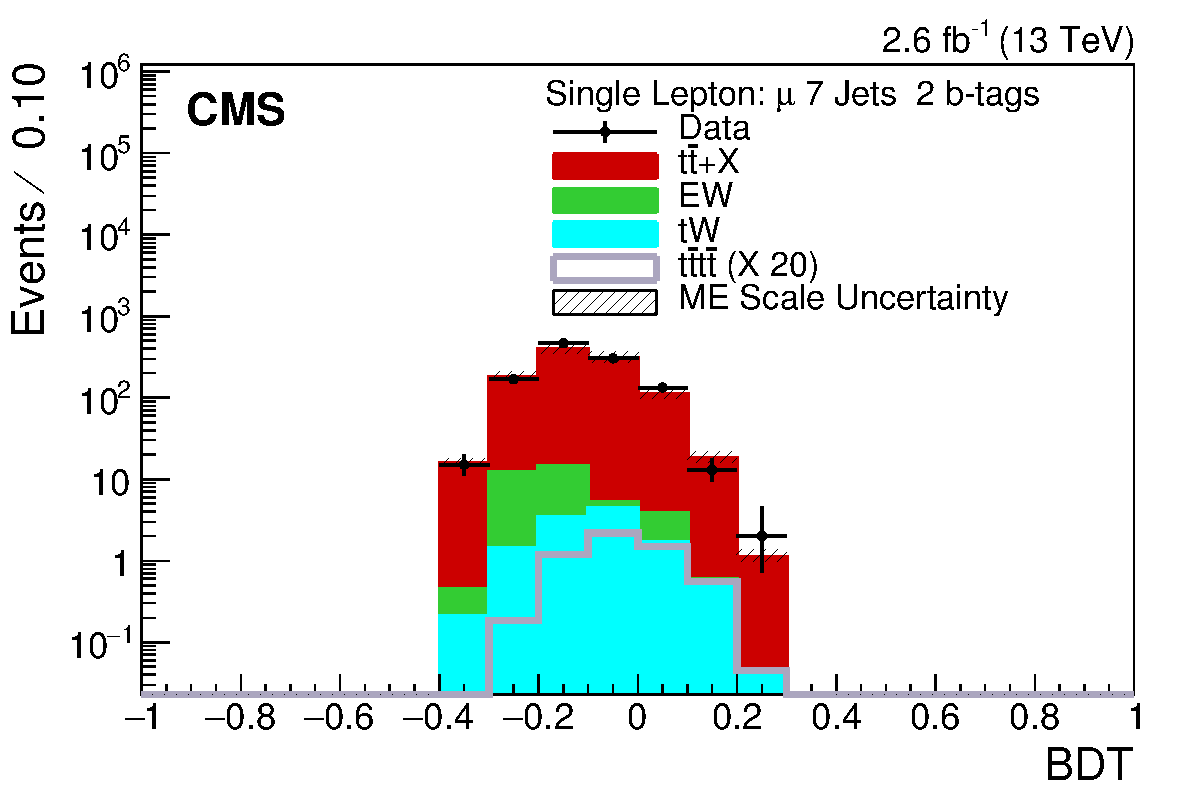
\includegraphics[width=0.48\textwidth]{images/Run2/BDT_Mu29Aug400trees_5MinNodeSize_20nCuts_3MaxDepth_5adaboostbeta_adaBoost_alphaSTune_noMinEvents7nJets2nMtags_StackLogY.pdf}
    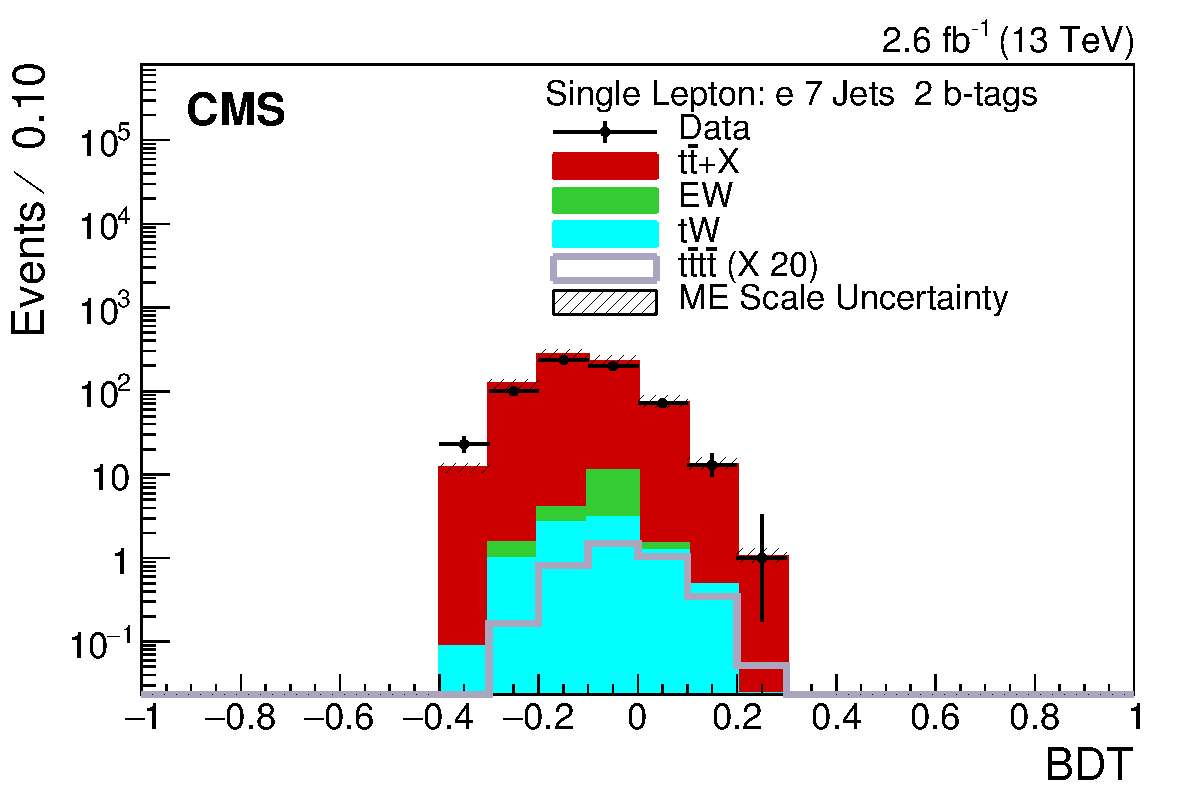
\includegraphics[width=0.48\textwidth]{images/Run2/BDT_El29Aug400trees_5MinNodeSize_20nCuts_3MaxDepth_5adaboostbeta_adaBoost_alphaSTune_noMinEvents7nJets2nMtags_StackLogY.pdf} 
    \caption{The BDT output distributions for AdaBoost for data and simulation in the $\mu$ + jets channel (left) and e + jets channel (left) are shown for the 7 \njets and 2 \nMtags category.}
    \label{fig:BDT_Mu29Aug400trees_5MinNodeSize_20nCuts_3MaxDepth_5adaboostbeta_adaBoost_alphaSTune_noMinEvents72}
 \end{figure}

\begin{figure}[ht!]
    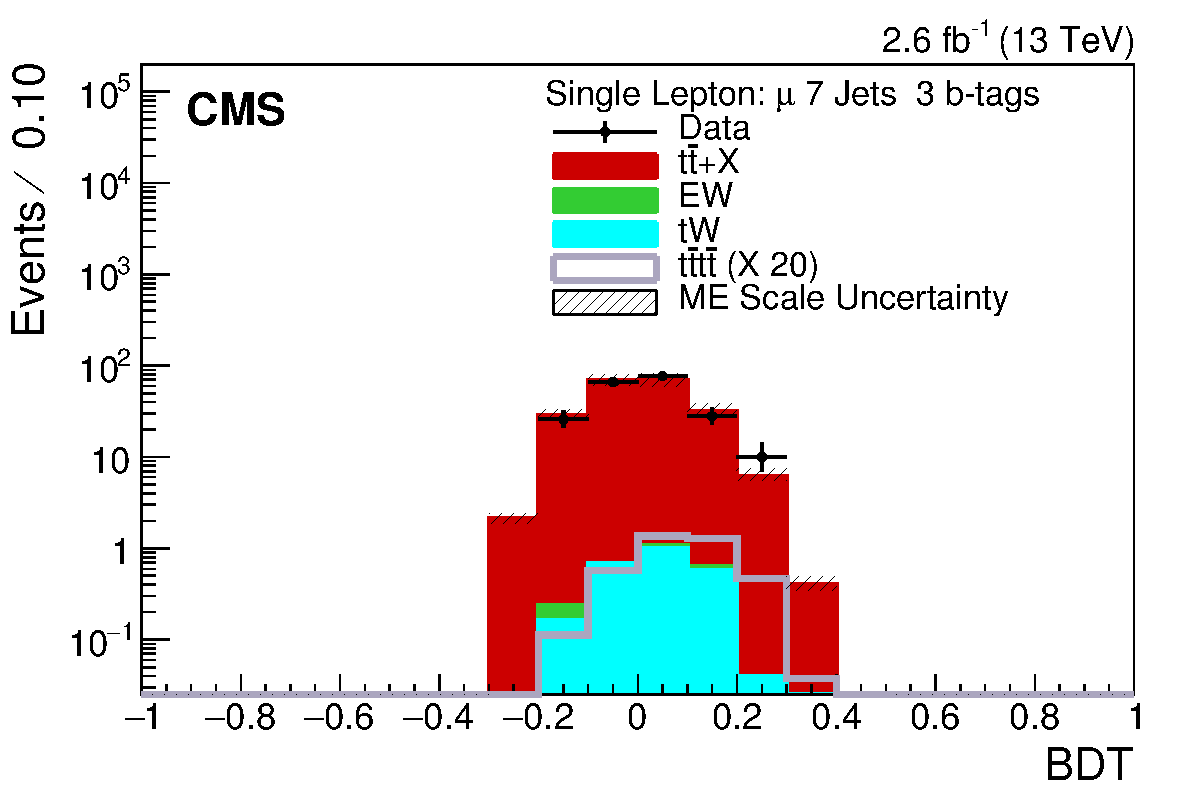
\includegraphics[width=0.48\textwidth]{images/Run2/BDT_Mu29Aug400trees_5MinNodeSize_20nCuts_3MaxDepth_5adaboostbeta_adaBoost_alphaSTune_noMinEvents7nJets3nMtags_StackLogY.pdf}
    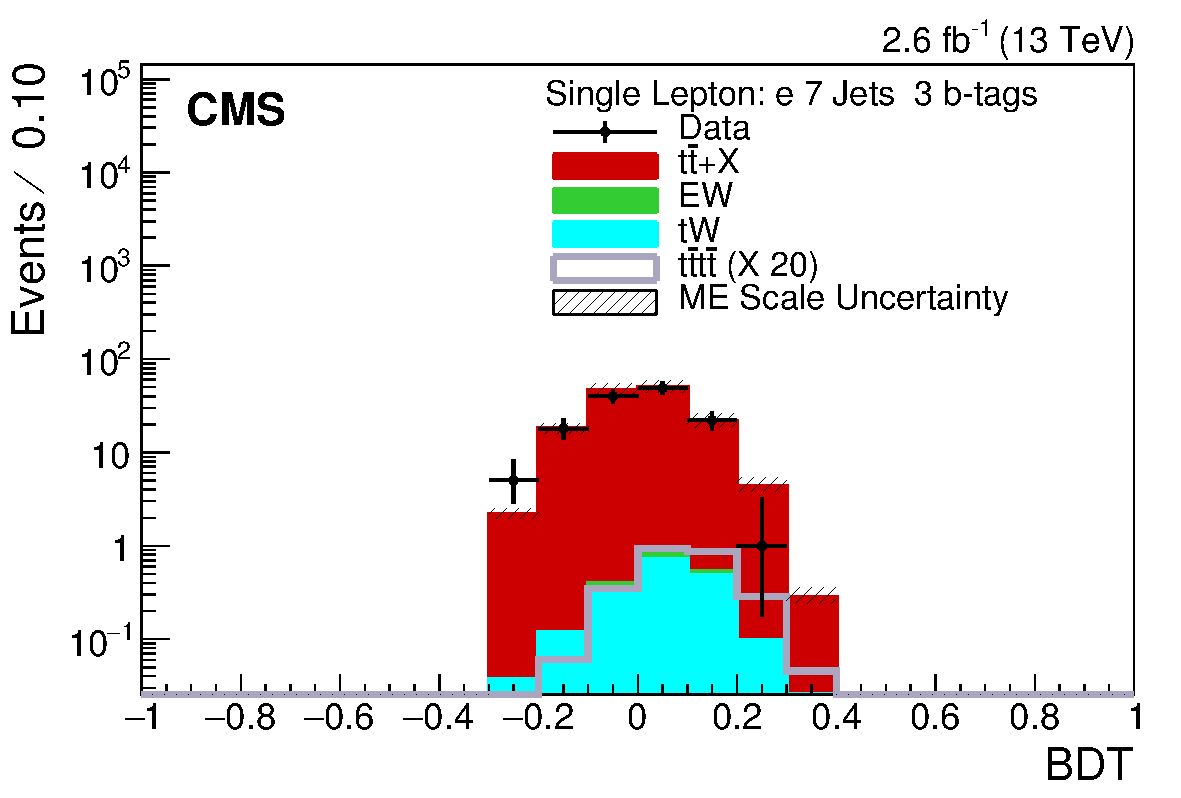
\includegraphics[width=0.48\textwidth]{images/Run2/BDT_El29Aug400trees_5MinNodeSize_20nCuts_3MaxDepth_5adaboostbeta_adaBoost_alphaSTune_noMinEvents7nJets3nMtags_StackLogY.pdf}
    \caption{The BDT output distributions for AdaBoost for data and simulation in the $\mu$ + jets channel (left) and e + jets channel (left) are shown for the 7 \njets and 3 \nMtags category.}
    \label{fig:BDT_Mu29Aug400trees_5MinNodeSize_20nCuts_3MaxDepth_5adaboostbeta_adaBoost_alphaSTune_noMinEvents73}
 \end{figure}

\begin{figure}[ht!]
    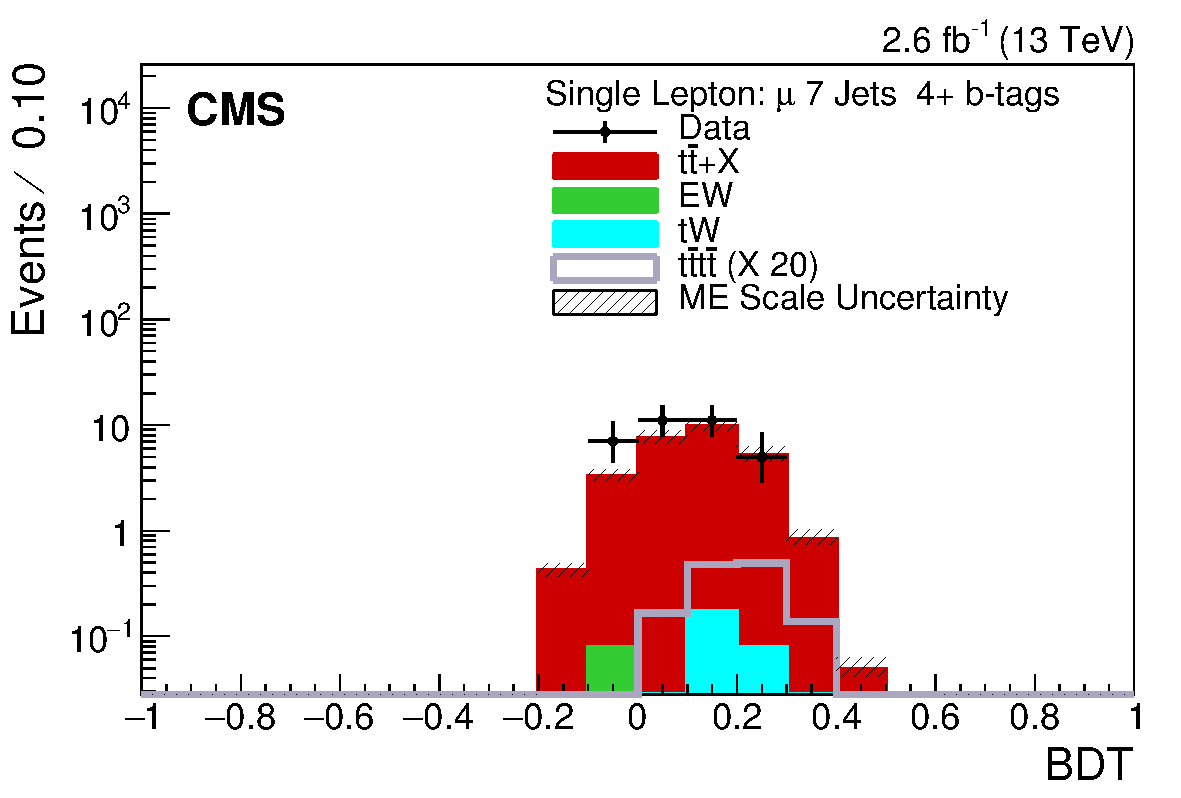
\includegraphics[width=0.48\textwidth]{images/Run2/BDT_Mu29Aug400trees_5MinNodeSize_20nCuts_3MaxDepth_5adaboostbeta_adaBoost_alphaSTune_noMinEvents7nJets4nMtags_StackLogY.pdf}
    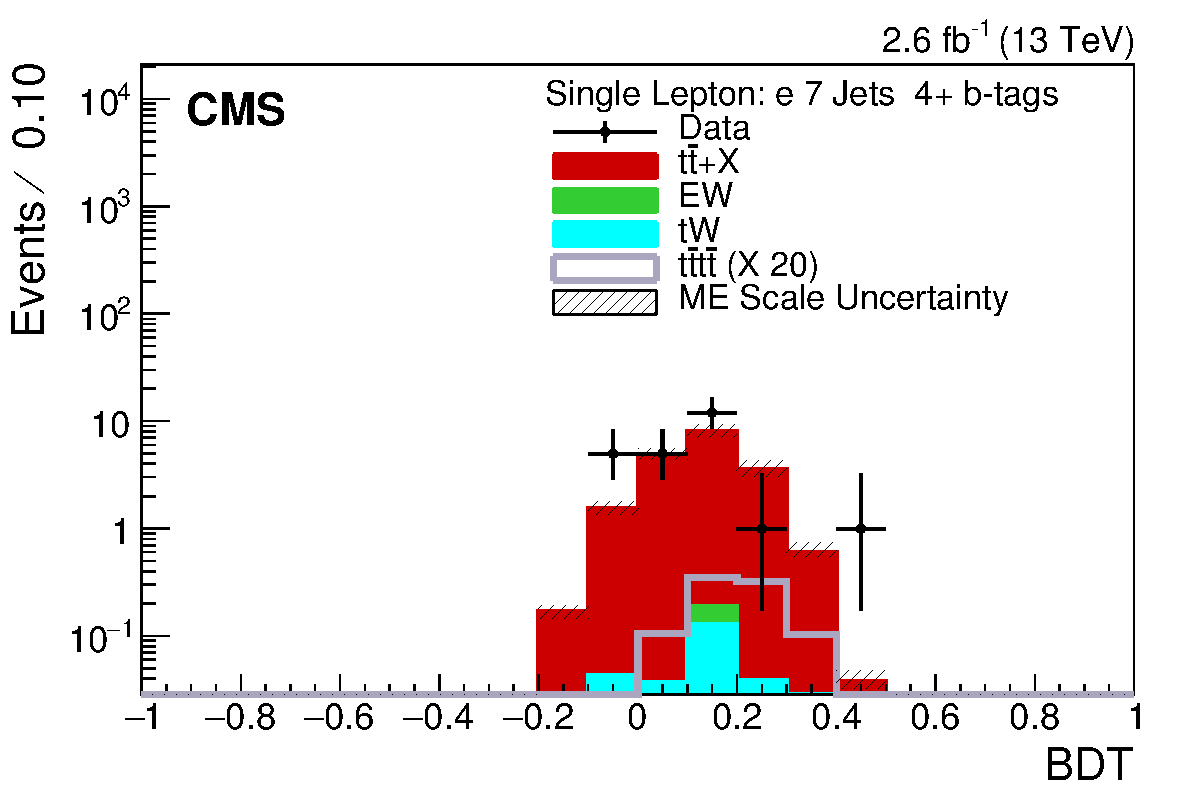
\includegraphics[width=0.48\textwidth]{images/Run2/BDT_El29Aug400trees_5MinNodeSize_20nCuts_3MaxDepth_5adaboostbeta_adaBoost_alphaSTune_noMinEvents7nJets4nMtags_StackLogY.pdf}
    \caption{The BDT output distributions for AdaBoost for data and simulation in the $\mu$ + jets channel (left) and e + jets channel (right) are shown for the 7 \njets and $\geq4$ \nMtags category.}
    \label{fig:BDT_Mu29Aug400trees_5MinNodeSize_20nCuts_3MaxDepth_5adaboostbeta_adaBoost_alphaSTune_noMinEvents74}
\end{figure}

\begin{figure}[ht!]
    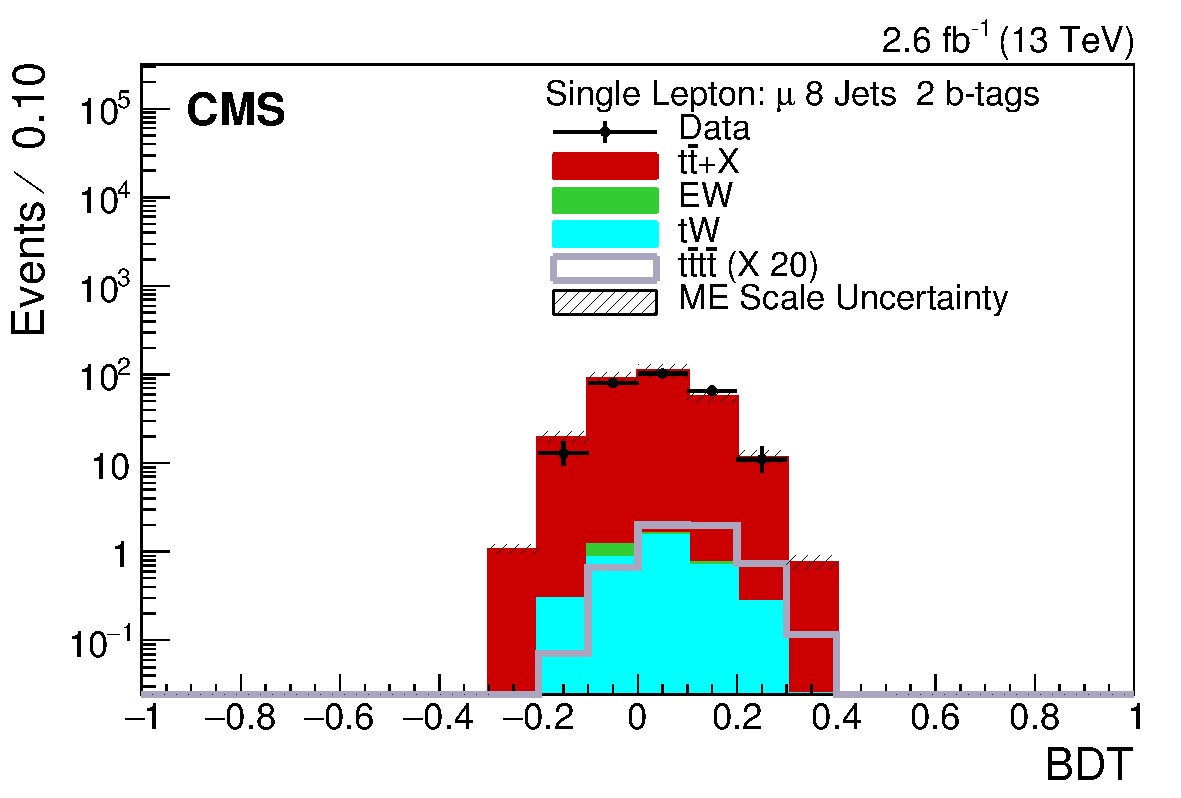
\includegraphics[width=0.48\textwidth]{images/Run2/BDT_Mu29Aug400trees_5MinNodeSize_20nCuts_3MaxDepth_5adaboostbeta_adaBoost_alphaSTune_noMinEvents8nJets2nMtags_StackLogY.pdf}
    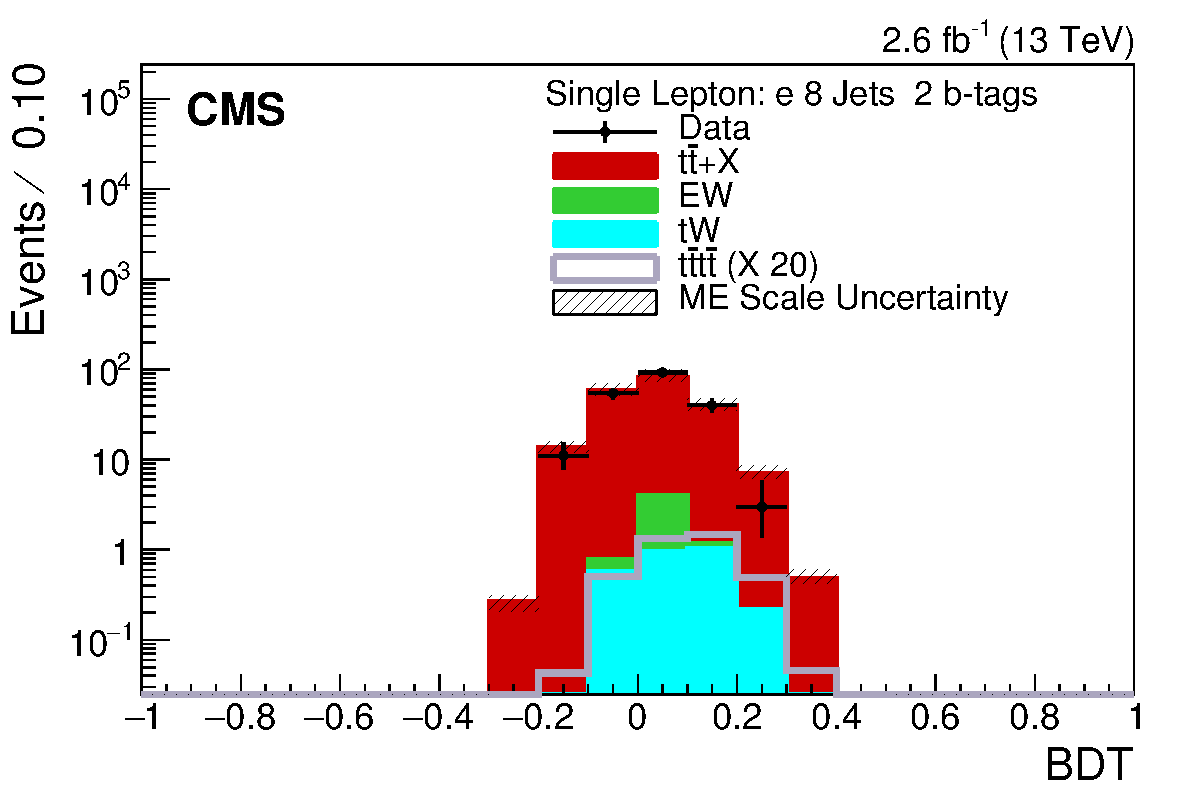
\includegraphics[width=0.48\textwidth]{images/Run2/BDT_El29Aug400trees_5MinNodeSize_20nCuts_3MaxDepth_5adaboostbeta_adaBoost_alphaSTune_noMinEvents8nJets2nMtags_StackLogY.pdf} 
    \caption{The BDT output distributions for AdaBoost for data and simulation in the $\mu$ + jets channel (left) and $e$ + jets channel (left) are shown for the 8 \njets and 2 \nMtags category.}
    \label{fig:BDT_Mu29Aug400trees_5MinNodeSize_20nCuts_3MaxDepth_5adaboostbeta_adaBoost_alphaSTune_noMinEvents82}
\end{figure}

\begin{figure}[ht!]
    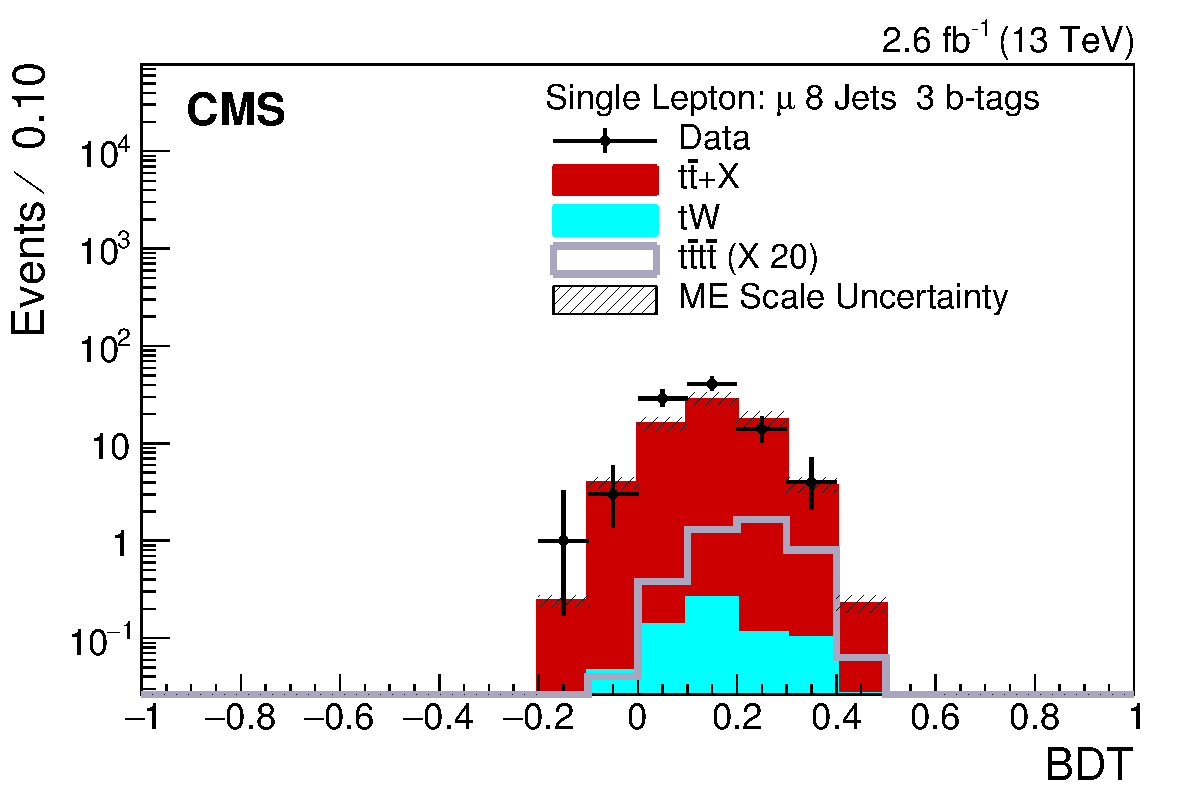
\includegraphics[width=0.48\textwidth]{images/Run2/BDT_Mu29Aug400trees_5MinNodeSize_20nCuts_3MaxDepth_5adaboostbeta_adaBoost_alphaSTune_noMinEvents8nJets3nMtags_StackLogY.pdf}
    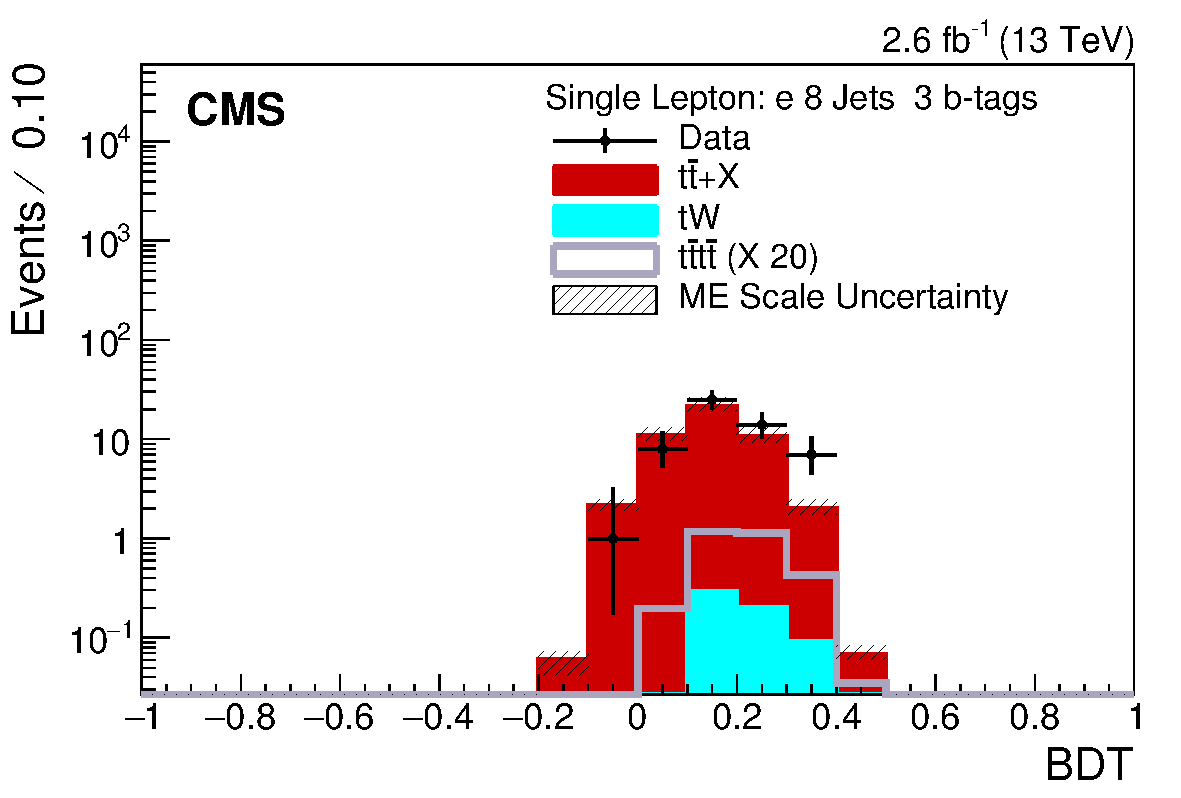
\includegraphics[width=0.48\textwidth]{images/Run2/BDT_El29Aug400trees_5MinNodeSize_20nCuts_3MaxDepth_5adaboostbeta_adaBoost_alphaSTune_noMinEvents8nJets3nMtags_StackLogY.pdf} 
    \caption{The BDT output distributions for AdaBoost for data and simulation in the $\mu$ + jets channel (left) and $e$ + jets channel (left) are shown for the 8 \njets category and 3 \nMtags category.}
    \label{fig:BDT_Mu29Aug400trees_5MinNodeSize_20nCuts_3MaxDepth_5adaboostbeta_adaBoost_alphaSTune_noMinEvents83}
\end{figure}

\begin{figure}[ht!]
    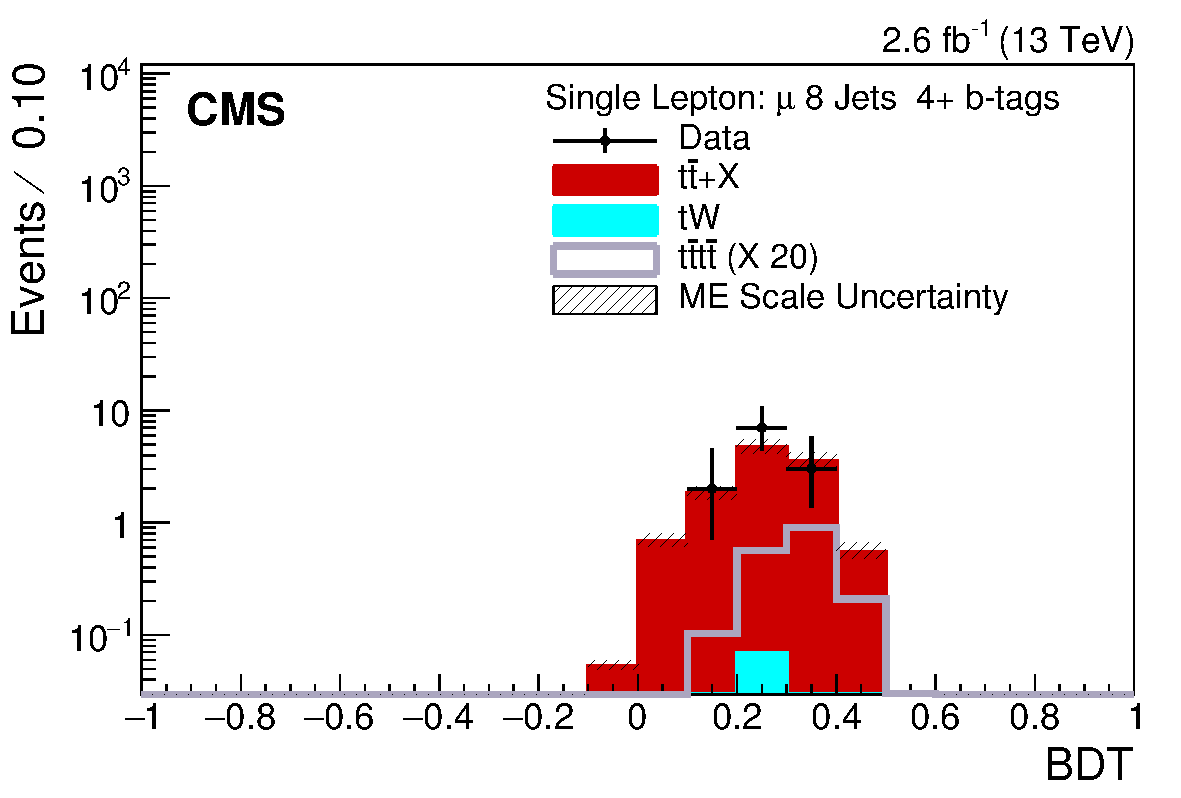
\includegraphics[width=0.48\textwidth]{images/Run2/BDT_Mu29Aug400trees_5MinNodeSize_20nCuts_3MaxDepth_5adaboostbeta_adaBoost_alphaSTune_noMinEvents8nJets4nMtags_StackLogY.pdf}
    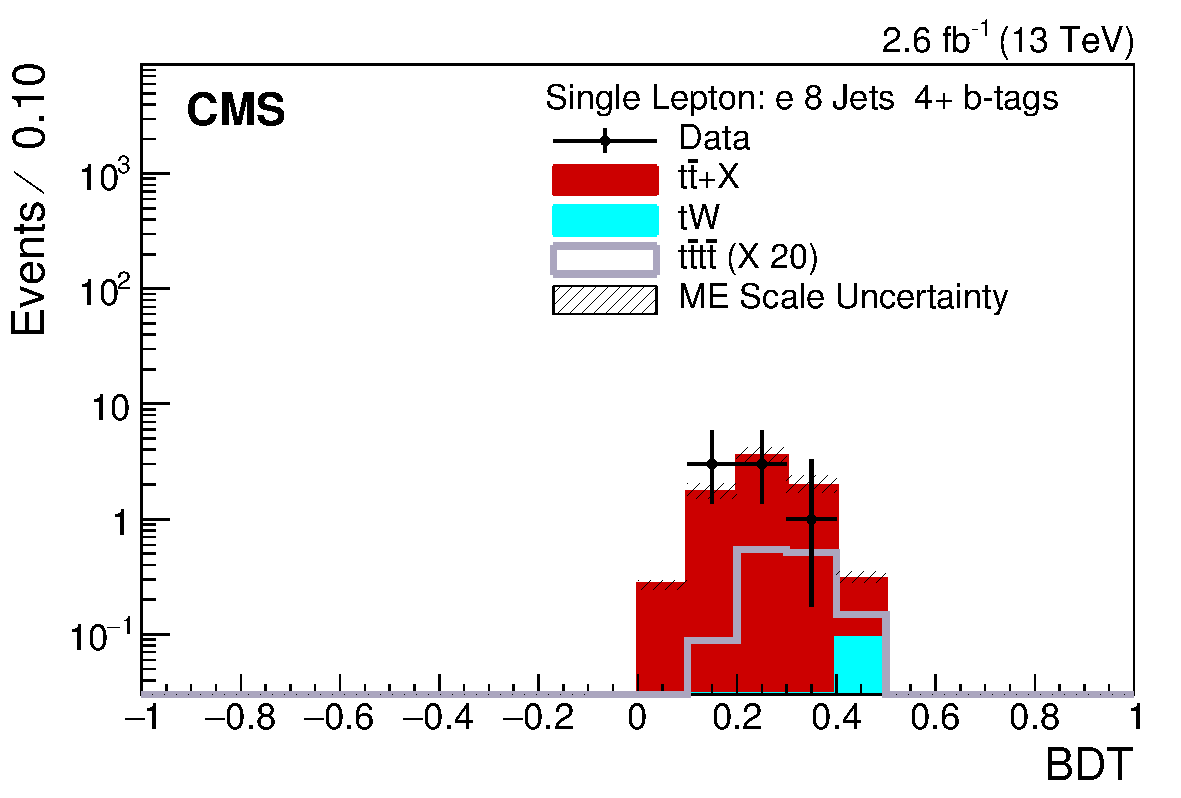
\includegraphics[width=0.48\textwidth]{images/Run2/BDT_El29Aug400trees_5MinNodeSize_20nCuts_3MaxDepth_5adaboostbeta_adaBoost_alphaSTune_noMinEvents8nJets4nMtags_StackLogY.pdf}
    \caption{The BDT output distributions for AdaBoost for data and simulation in the $\mu$ + jets channel (left) and $e$ + jets channel (right) are shown for the 8 \njets and $\geq4$ \nMtags category.}
    \label{fig:BDT_Mu29Aug400trees_5MinNodeSize_20nCuts_3MaxDepth_5adaboostbeta_adaBoost_alphaSTune_noMinEvents84}
\end{figure}

\newpage

\begin{figure}[ht!]
    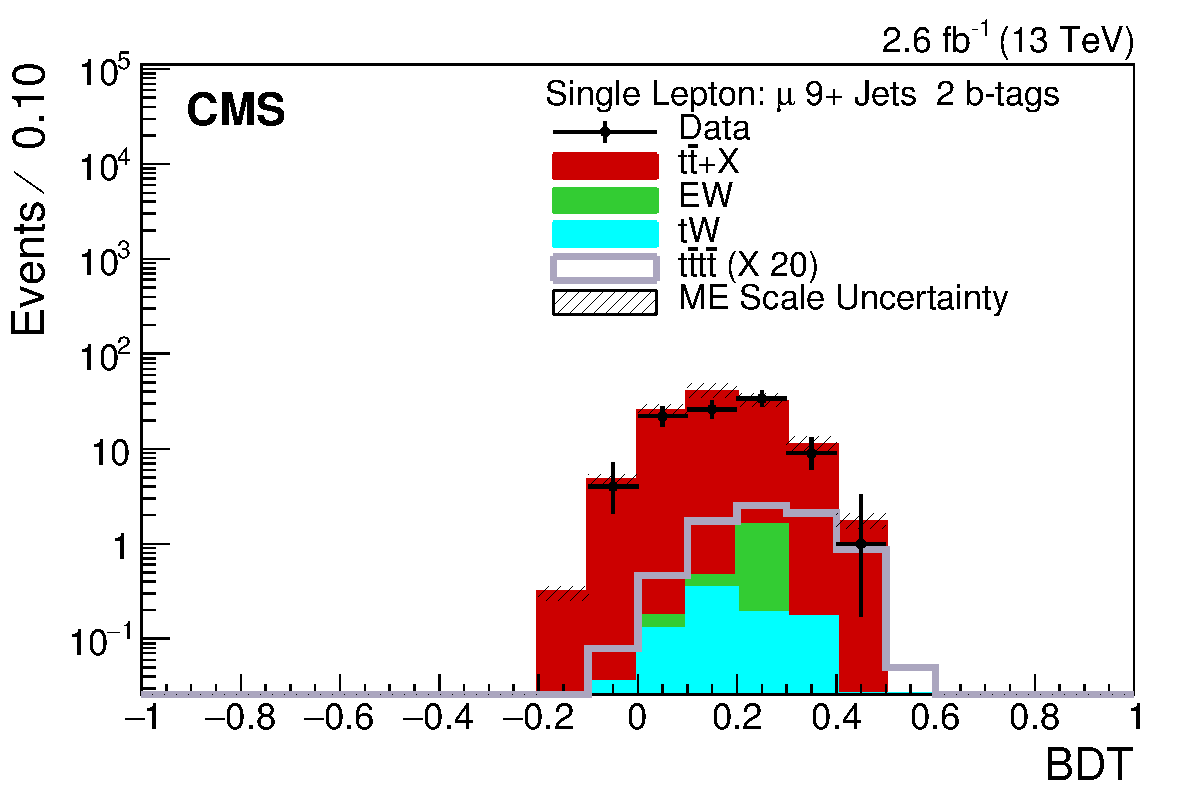
\includegraphics[width=0.48\textwidth]{images/Run2/BDT_Mu29Aug400trees_5MinNodeSize_20nCuts_3MaxDepth_5adaboostbeta_adaBoost_alphaSTune_noMinEvents9nJets2nMtags_StackLogY.pdf}
    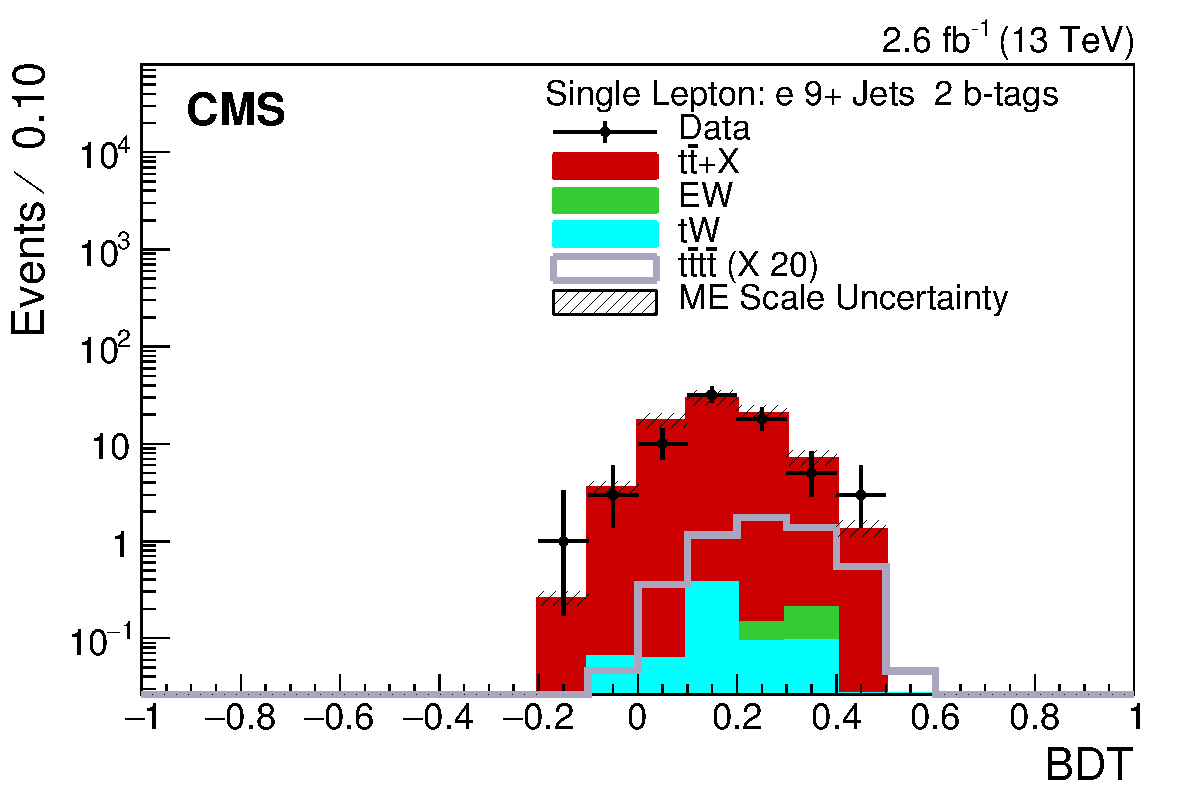
\includegraphics[width=0.48\textwidth]{images/Run2/BDT_El29Aug400trees_5MinNodeSize_20nCuts_3MaxDepth_5adaboostbeta_adaBoost_alphaSTune_noMinEvents9nJets2nMtags_StackLogY.pdf} 
    \caption{The BDT output distributions for AdaBoost for data and simulation in the $\mu$ + jets channel (left) and $e$ + jets channel (left) are shown for the $\geq9$ \njets  and 2 \nMtags category.}
    \label{fig:BDT_Mu29Aug400trees_5MinNodeSize_20nCuts_3MaxDepth_5adaboostbeta_adaBoost_alphaSTune_noMinEvents92}
\end{figure}

\begin{figure}[ht!]
    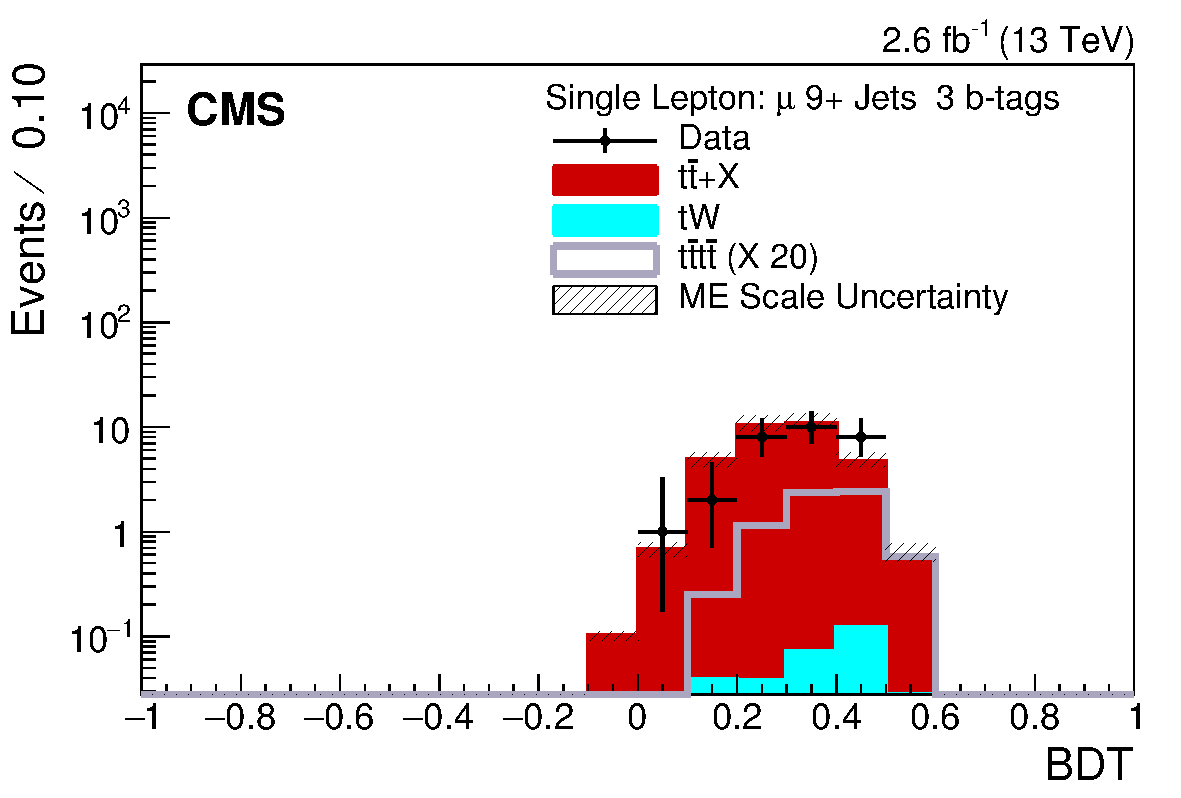
\includegraphics[width=0.48\textwidth]{images/Run2/BDT_Mu29Aug400trees_5MinNodeSize_20nCuts_3MaxDepth_5adaboostbeta_adaBoost_alphaSTune_noMinEvents9nJets3nMtags_StackLogY.pdf}
    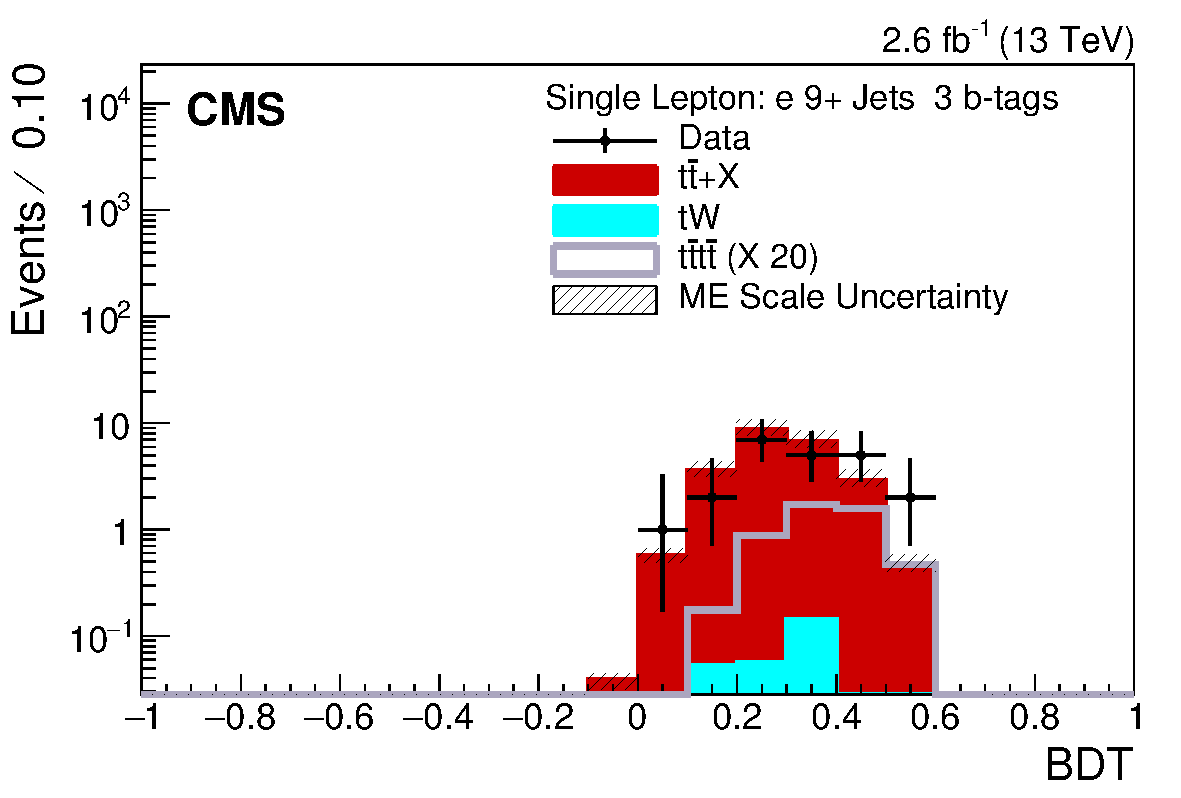
\includegraphics[width=0.48\textwidth]{images/Run2/BDT_El29Aug400trees_5MinNodeSize_20nCuts_3MaxDepth_5adaboostbeta_adaBoost_alphaSTune_noMinEvents9nJets3nMtags_StackLogY.pdf}
    \caption{The BDT output distributions for AdaBoost for data and simulation in the $\mu$ + jets channel (left) and $e$ + jets channel (left) are shown for the $\geq9$ \njets  and 3 \nMtags category.}
    \label{fig:BDT_Mu29Aug400trees_5MinNodeSize_20nCuts_3MaxDepth_5adaboostbeta_adaBoost_alphaSTune_noMinEvents93}
\end{figure}

\begin{figure}[ht!]
    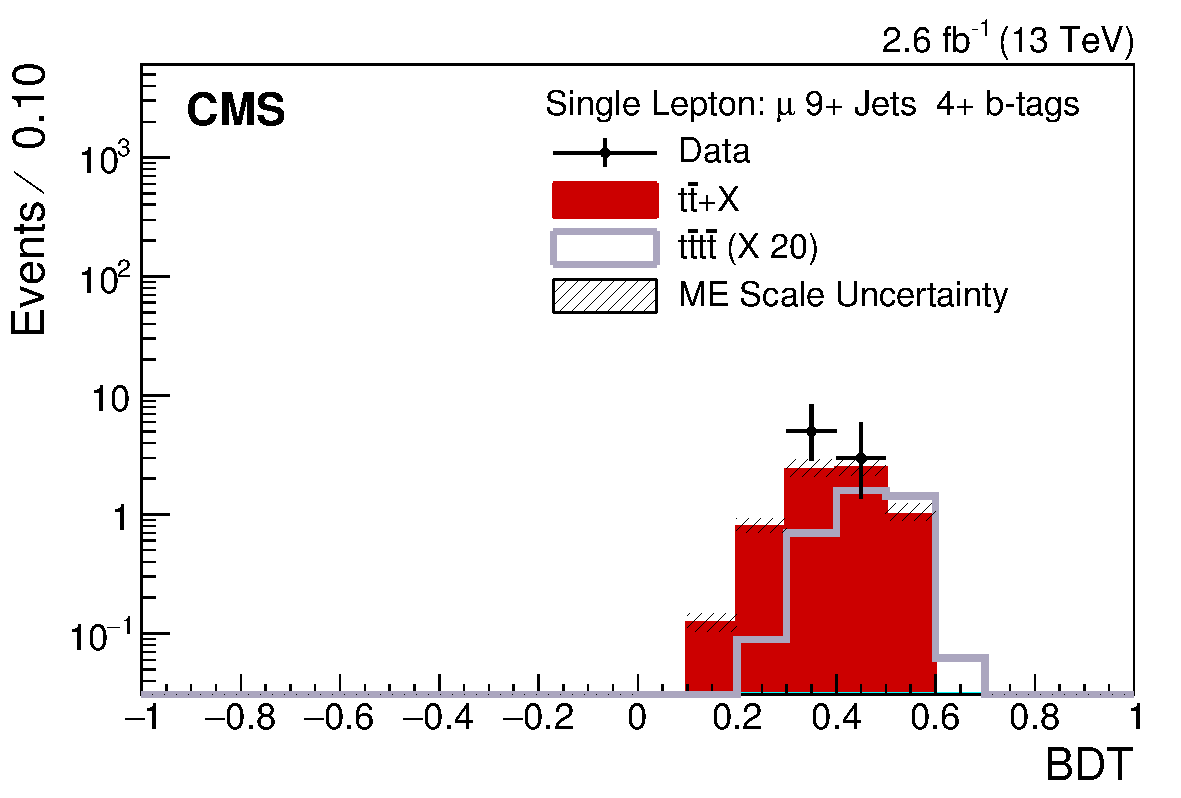
\includegraphics[width=0.48\textwidth]{images/Run2/BDT_Mu29Aug400trees_5MinNodeSize_20nCuts_3MaxDepth_5adaboostbeta_adaBoost_alphaSTune_noMinEvents9nJets4nMtags_StackLogY.pdf}
    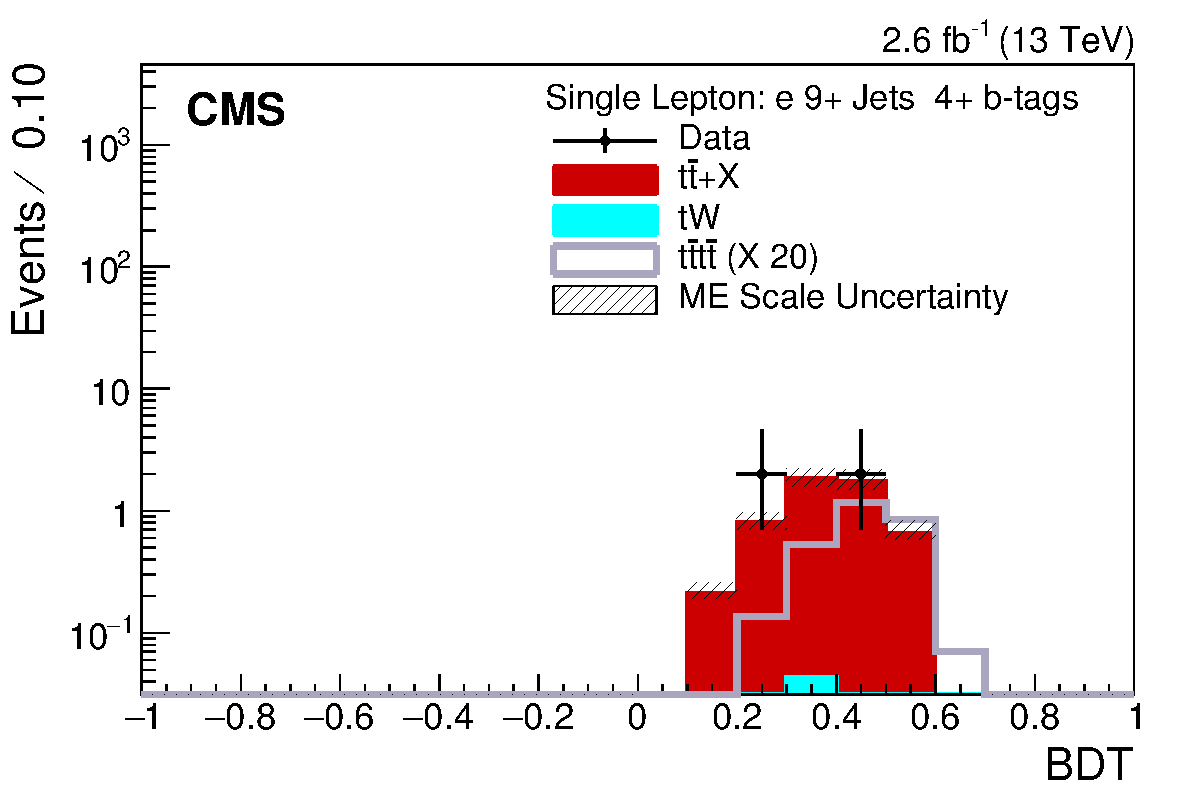
\includegraphics[width=0.48\textwidth]{images/Run2/BDT_El29Aug400trees_5MinNodeSize_20nCuts_3MaxDepth_5adaboostbeta_adaBoost_alphaSTune_noMinEvents9nJets4nMtags_StackLogY.pdf}    
    \caption{The BDT output distributions for AdaBoost for data and simulation in the $\mu$ + jets channel (left) and $e$ + jets channel (right) are shown for the $\geq9$ \njets and $\geq4$ \nMtags category.}
    \label{fig:BDT_Mu29Aug400trees_5MinNodeSize_20nCuts_3MaxDepth_5adaboostbeta_adaBoost_alphaSTune_noMinEvents94}
\end{figure}

\section{Systematic uncertainties}
\label{sec:uncertainties13}
All systematic uncertainties are described in section~\ref{sec:uncertainties} and some further details about them are given below.

\begin{itemize}
\item \textbf{Luminosity}\\
The CMS Luminosity Group gave a recommendation of 2.7$\%$ uncertainty on the luminosity~\cite{CMS-PAS-LUM-15-001} which is applied to all backgrounds.
\item \textbf{Monte Carlo cross sections}\\
The uncertainty on main background of \ttbar is ${}^{+2.5\%}_{-3.4\%}$ renormalisation and factorisation scale and ${}^{+6.2\%}_{-6.4\%} \left( \textrm{PDF} \right)$~\cite{PhysRevLett.110.252004}. The MC cross section uncertainties for the other background processes are modelled by assigning a $4\%$ uncertainty and a $10\%$ uncertainty is assigned to the signal process.
\item \textbf{Lepton SF}\\
Applied to all backgrounds. 1.3$\%$ in muon channel and 3.6$\%$ in electron channel
\item \textbf{Matrix Element Factorisation and renormalisation scales}\\
Weights are available in the \ttbar and \tttt samples which correspond to the factorisation and renormalisation scale $\left(\mu_{f},~\mu_{s}\right)$ being individually varied through 1/2~u, u and 2~u, where u represents the central value. This give nine weights however the extreme unphysical values of (1/2~u, 1/2~u) and (2~u, 2~u) are not included. Applying these weights individually gives six alternative event-level BDT histograms to the central histogram, which uses (u,u). 
\item \textbf{Parton Shower Factorisation and renormalisation scales}\\
The effect of the parton showering scale in the \PYTHIA~8 generator is evaluated by using alternative \ttbar samples with the PS scale (u$_{PS}$) varied by 2~u$_{PS}$, 1/2~u$_{PS}$. This shift in the PS scale is equivalent to modifying the value of $\alpha_{S}$ hence the alternative parton shower histogram shapes have been inflated by a factor of 1.5 relative to the nominal template to take into account the uncertainty on the jet multiplicity modelling.
\item \textbf{\ttbar generator}\\
The \POWHEG generator was used to produce the nominal \ttbar sample for this analysis. This can be compared to running the analysis with the \MLM and \MADGRAPH\aMCATNLO~FxFx \ttbar samples. A symmetric envelope could be formed around the nominal by symmetrising the difference in event counts in each bin between the alternative and nominal samples. The \MLM sample was found to produce the most conservative uncertainty for this effect and so it was used to produce the symmetric up and down histograms.
\item \textbf{JES}\\
The JES uncertainty is derived by varying the JES by $\pm1\sigma$ for the \ttbar and \tttt samples.
\item \textbf{JER}\\
The JER uncertainty is derived by varying the smearing by $\pm1\sigma$ for the \ttbar and \tttt samples.
\item \textbf{b tagging}\\
As detailed in Section~\ref{sec:Calibrations13} the difference between b-tagging efficiency in data and simulation is accounted for by the application of scale factors to simulated events via an event weighting procedure. This is the event weighting procedure used by the \ttH analysis~\cite{CMS-PAS-HIG-16-004}, details of which are documented here~\cite{CMS-NOTE-2013-130}. Given the significant uncertainty on these scale factors and that the CSV distributions are input variables to the BDT algorithm, a significant systematic effect is expected. Light flavour, `lf', and linear statistical and quadratic statistical fluctuations, `hfstats1' and `hfstats2', are applied to heavy flavour jets.  Heavy flavour, `hf', and linear statistical and quadratic statistical fluctuations, `lfstats1' and `lfstats2', are applied to light flavour jets. Linear and quadratic uncertainties, `cferr1' and `cferr2', are applied to charm flavour jets. A b-tagging JES systematic is applied to light and heavy flavour jets when the standard jet energy scale systematics are applied and hence it is incorporated into the alternative JES systematic shapes. The b-tagging systematic is studied for the \ttbar and \tttt samples.
\item \textbf{Pile up}\\
The PU systematic uncertainty is found by varying the MinBias cross section by $\pm5\%$ and is applied to the \ttbar and \tttt samples.
\item \textbf{\heavyflavourone / \heavyflavourtwo modelling}
The uncertainty on the measurement of \heavyflavourone / \heavyflavourtwo by CMS~\cite{Khachatryan2015132} is $\pm 0.3 \left( \textrm{stat.} \right) \pm 0.6 \left(\textrm{sys.} \right)$. Alternative event weights are derived for \heavyflavourone / \heavyflavourtwo which are used to provide the alternative systematic up and down histograms.
\end{itemize}
\section{Template fit and upper limit}
\label{sec:limit13}
As no excess of events over the background expectation consistent with SM $\tttt$ production was observed, upper limits on $\sigma_{\tttt}^{SM}$ are calculated. 
The limit setting proceeds by simultaneously fitting the BDT output distributions of signal and backgrounds to the BDT distribution of data in both the $\mu$ + jets and $e$ + jets channels in all 12 \njets and \nMtags categories. The Higgs Combined Tool is used to perform the fit, assigning lognormal uncertainties to normalisation systematic uncertainties and the vertical morphing technique described in Section~\ref{sec:limitFit} for the shape systematic uncertainties. The fit produces a fitted shape and normalisation and best-fit values for all nuisance parameters and the parameter of interest. 
To avoid prohibitively large computing times, the approximate \emph{asymptotic} approach is used to calculate the \CLS limits, which can be found in table~\ref{tab:limits} in unit of $\sigma_{SM}$. 

\begin{table}[ht!]
\centering
\begin{tabular}{| l | c | c | c | c | c |}
  \hline
Channel  & Categorized & Uncertainty & Observed\\
 \hline
$\mu$  &$20.6$ & $+12.9 -7.2$ & $20.8$ \\
 \hline
e  &  $26.4$ & $+16.6 -9.3$ & $33.5$ \\
 \hline
 Combined  &  $16.0$ & $+9.8 -5.5$ & $16.8$ \\
 \hline
\end{tabular}
 \caption{Extracted expected limits for \njets and \nMtags categorized templates in multiples of $\sigma_{SM}$.}
  \label{tab:limits}
  \end{table}

The combined expected limit is $147.2^{+90}_{-51}$~fb and the observed limit is 154.6~fb for the single lepton + jets channel.

\section{Systematics studies and tests on analysis}

\section{Combination with OS dilepton channel and SS dilepton channel}

The sensitivity of the search for standard model four top quark production can be improved by combining with other search channels. An opposite-sign (OS) search was developed in parallel with the single lepton channel study described in this chapter~\cite{CMS-PAS-TOP-16-016}. The analysis selects on events which contain any combination of $\mu^{+}\mu^{-}$, $\mu^{\pm} e^{\mp}$, $e^{+}e^{-}$. It uses the same hadronic top quark reconstruction as in Section~\ref{sec:topContent13} to identify the BDT value for highest-ranked top quark candidate, $BDT_{trijet1}$. This variable is fed into the event-level BDT along with other variables based on the event-topology, event activity and b-jet content. A simultaneous fit was made using the BDT histogram templates described above for the single lepton channel and the BDT histogram templates (which are split only in \njets categories due to statistical limitations) from the dilepton channel. All systematic uncertainties apart from the lepton scale factors were treated as correlated. The results of this fit can be found in table~\ref{tab:limits_combined} in the row labelled \emph{Combined (single lepton and OS dilepton)}. It is clear that the OS dilepton channel alone is not as sensitive as the single lepton channel, which is due in part to it having a smaller branching ratio, however it's combination with the single lepton channel improves the overall sensitivity.\\

The analysis was then further combined with a search for new physics in events with same-sign (SS) dileptons which places limits on the standard model production of four top quarks~\cite{Khachatryan:2016kod}. This search benefits from very low numbers of events from background processes which gives rise to it's good signal sensitivity. The luminosity, JES and PU systematic uncertainties were treated correlated between the SS dilepton channel and the other two channels. The uncertainty in response of the CMS trigger system to events containing dileptons is was also treated as correlated between the two dilepton analyses, whilst all other systematic uncertainties were treated as fully uncorrelated between the SS dilepton analysis and the other two search channels. The combination of all channels is listed in Table~\ref{tab:limits_combined} where it can be seen that this gives a significant improvement in the expected limit compared to any individual channel.

\begin{table}[ht!]
%NOTE: THE VALUES ARE DEFINED IN THE TOP-16-016.tex at the start - modify them there, not here.
    \caption{Expected and observed 95\% CL upper limits on the SM \tttt production as a multiple of \sigmattttSM and in fb. The values quoted on the expected limits are the $1$ standard deviation uncertainties and include all statistical and systematic uncertainties.}    
    \centering
    \small
    \begin{tabular}{ l | c  |  c | c  | c }
        Channel  & Expected Limit  & Observed Limit & Expected limit  & Observed Limit \T \B\\  
         & (x \sigmattttSM) & (x \sigmattttSM) & (fb) & (fb) \T \B \\ \hline 
                Single lepton  & $\xsecmusingleptonexp^{\,+\,\xsecmusingleptonup}_{\,-\,\xsecmusingleptondown}$ & $\xsecmusinglepton$ & $\xsecfbsingleptonexp^{\,+\,\xsecfbsingleptonup}_{\,-\,\xsecfbsingleptondown}$ & $\xsecfbsinglepton$   \T \B  \\ 
                  & & & &  \\

                Dilepton  & $\xsecmudileptonexp^{\,+\,\xsecmudileptonup}_{\,-\,\xsecmudileptondown}$ & $\xsecmudilepton$ & $\xsecfbdileptonexp^{\,+\,\xsecfbdileptonup}_{\,-\,\xsecfbdileptondown}$ & $\xsecfbdilepton$ \T \B   \\ 
                (opposite sign) & & & &  \\
            \hline 
                 Combined  & $\xsecmucomboexp^{\,+\,\xsecmucomboup}_{\,-\,\xsecmucombodown}$ & $\xsecmucombo$  & $\xsecfbcomboexp^{\,+\,\xsecfbcomboup}_{\,-\,\xsecfbcombodown}$ & $\xsecfbcombo$   \T \B  \\
                (this analysis) & & & &  \\   \hline \hline            
                Dilepton & $11.0^{\,+\,6.2}_{\,-\,3.8}$ & $12.9$ & $101^{\,+\,57}_{\,-\,35}$ & $119$   \T \B  \\
                (same sign) & & &  & \\ \hline
                Combined  & $\xsecmucomboallexp^{\,+\,\xsecmucomboallup}_{\,-\,\xsecmucomboalldown}$ & $\xsecmucomboall$  & $\xsecfbcomboallexp^{\,+\,\xsecfbcomboallup}_{\,-\,\xsecfbcomboalldown}$ & $\xsecfbcomboall$  \T \B   \\
                (all channels) & & & &  \\                
    \end{tabular}
    \label{tab:limits_combined}
\end{table}

\section{Summary and conclusion}
\label{sec:summary13}

\section{Discussion of ATLAS four-top-quark production studies at $\sqrt{s} =$~13~TeV}
\label{sec:ATLASresult13}
% \fxnote{Possible comparison with atlas requirements put into our framework}
